\documentclass{article}
\usepackage[utf8]{inputenc}
\usepackage{longtable} % for tables
\usepackage{graphicx} % for tables
\usepackage[a4paper,left=20mm,right=20mm, top=3cm, bottom=3cm]{geometry}
\usepackage{lscape}
\usepackage{hyperref}
\usepackage{subcaption}
\usepackage{caption}
\usepackage[table,xcdraw]{xcolor} % for tables
\usepackage{multirow} % for tables

\graphicspath{ {figures/} }

\title{African Genome Diversity Reference Panel and Chip Design}
\author{Tommy Carstensen, Deepti Gurdasani, Martin Pollard, Cristina Pomilla}
\date{January 2015}

\begin{document}

\maketitle
\centerline{
\includegraphics[width=80mm]{sang_logo_large}}

\section{Rationale}

With next generation genotyping, and the decline in genotyping costs, it has now become possible to carry out large-scale dense genotyping across individuals for genome wide association studies. While these chip designs capture variation in European populations very well, their utility in capturing variation in more diverse African populations is unclear. Using the African Genome Variation Project resource (AGVP), we have shown that existing chip designs with imputation using large-scale sequencing panels can capture common variation well relative to low coverage sequencing designs. We also show marked improvement in imputation accuracy, even for common variation, with addition of diverse African populations in imputation panels.\cite{Gurdasani2014}

We hypothesise that development of more efficient chip designs specific to African populations would complement the development of novel reference panels, and improve efficiency of variant capture by genotyping arrays even further. While existing chip designs have included African populations in the ascertainment set, European populations have dominated development of these arrays, and African populations in current reference panels are not representative of more differentiated population groups within Africa. Here, we describe the development of such an array, ascertained on large samples from distinct representative population groups across Africa.
\section{Summary of Datasets}
The chip design will incorporate several population groups collated from different parts of Africa. These include samples collated as part of the AGVP\cite{Gurdasani2014}, the 1000 Genomes project (\href{http://www.1000genomes.org}{http://www.1000genomes.org}),
% the Genome Diversity in Africa Project (GDAP),
% the Simon’s Foundation (\href{http://www.simonsfoundation.org/life-sciences/simons-genome-diversity-project-dataset/}{http://www.simonsfoundation.org/life-sciences/simons-genome-diversity-project-dataset/}),
 and other shared or publicly available data. These samples have been chosen to be representative of diverse ethnolinguistic and geographical groups across Africa. All samples will constitute the reference panel described in the tag SNP selection section, but tag SNPs will only be selected from populations with 50 samples or more. The chip efficiency will be validated with the remaining populations.

\begin{figure}[h]
\begin{subfigure}{.5\textwidth}
  \centering
  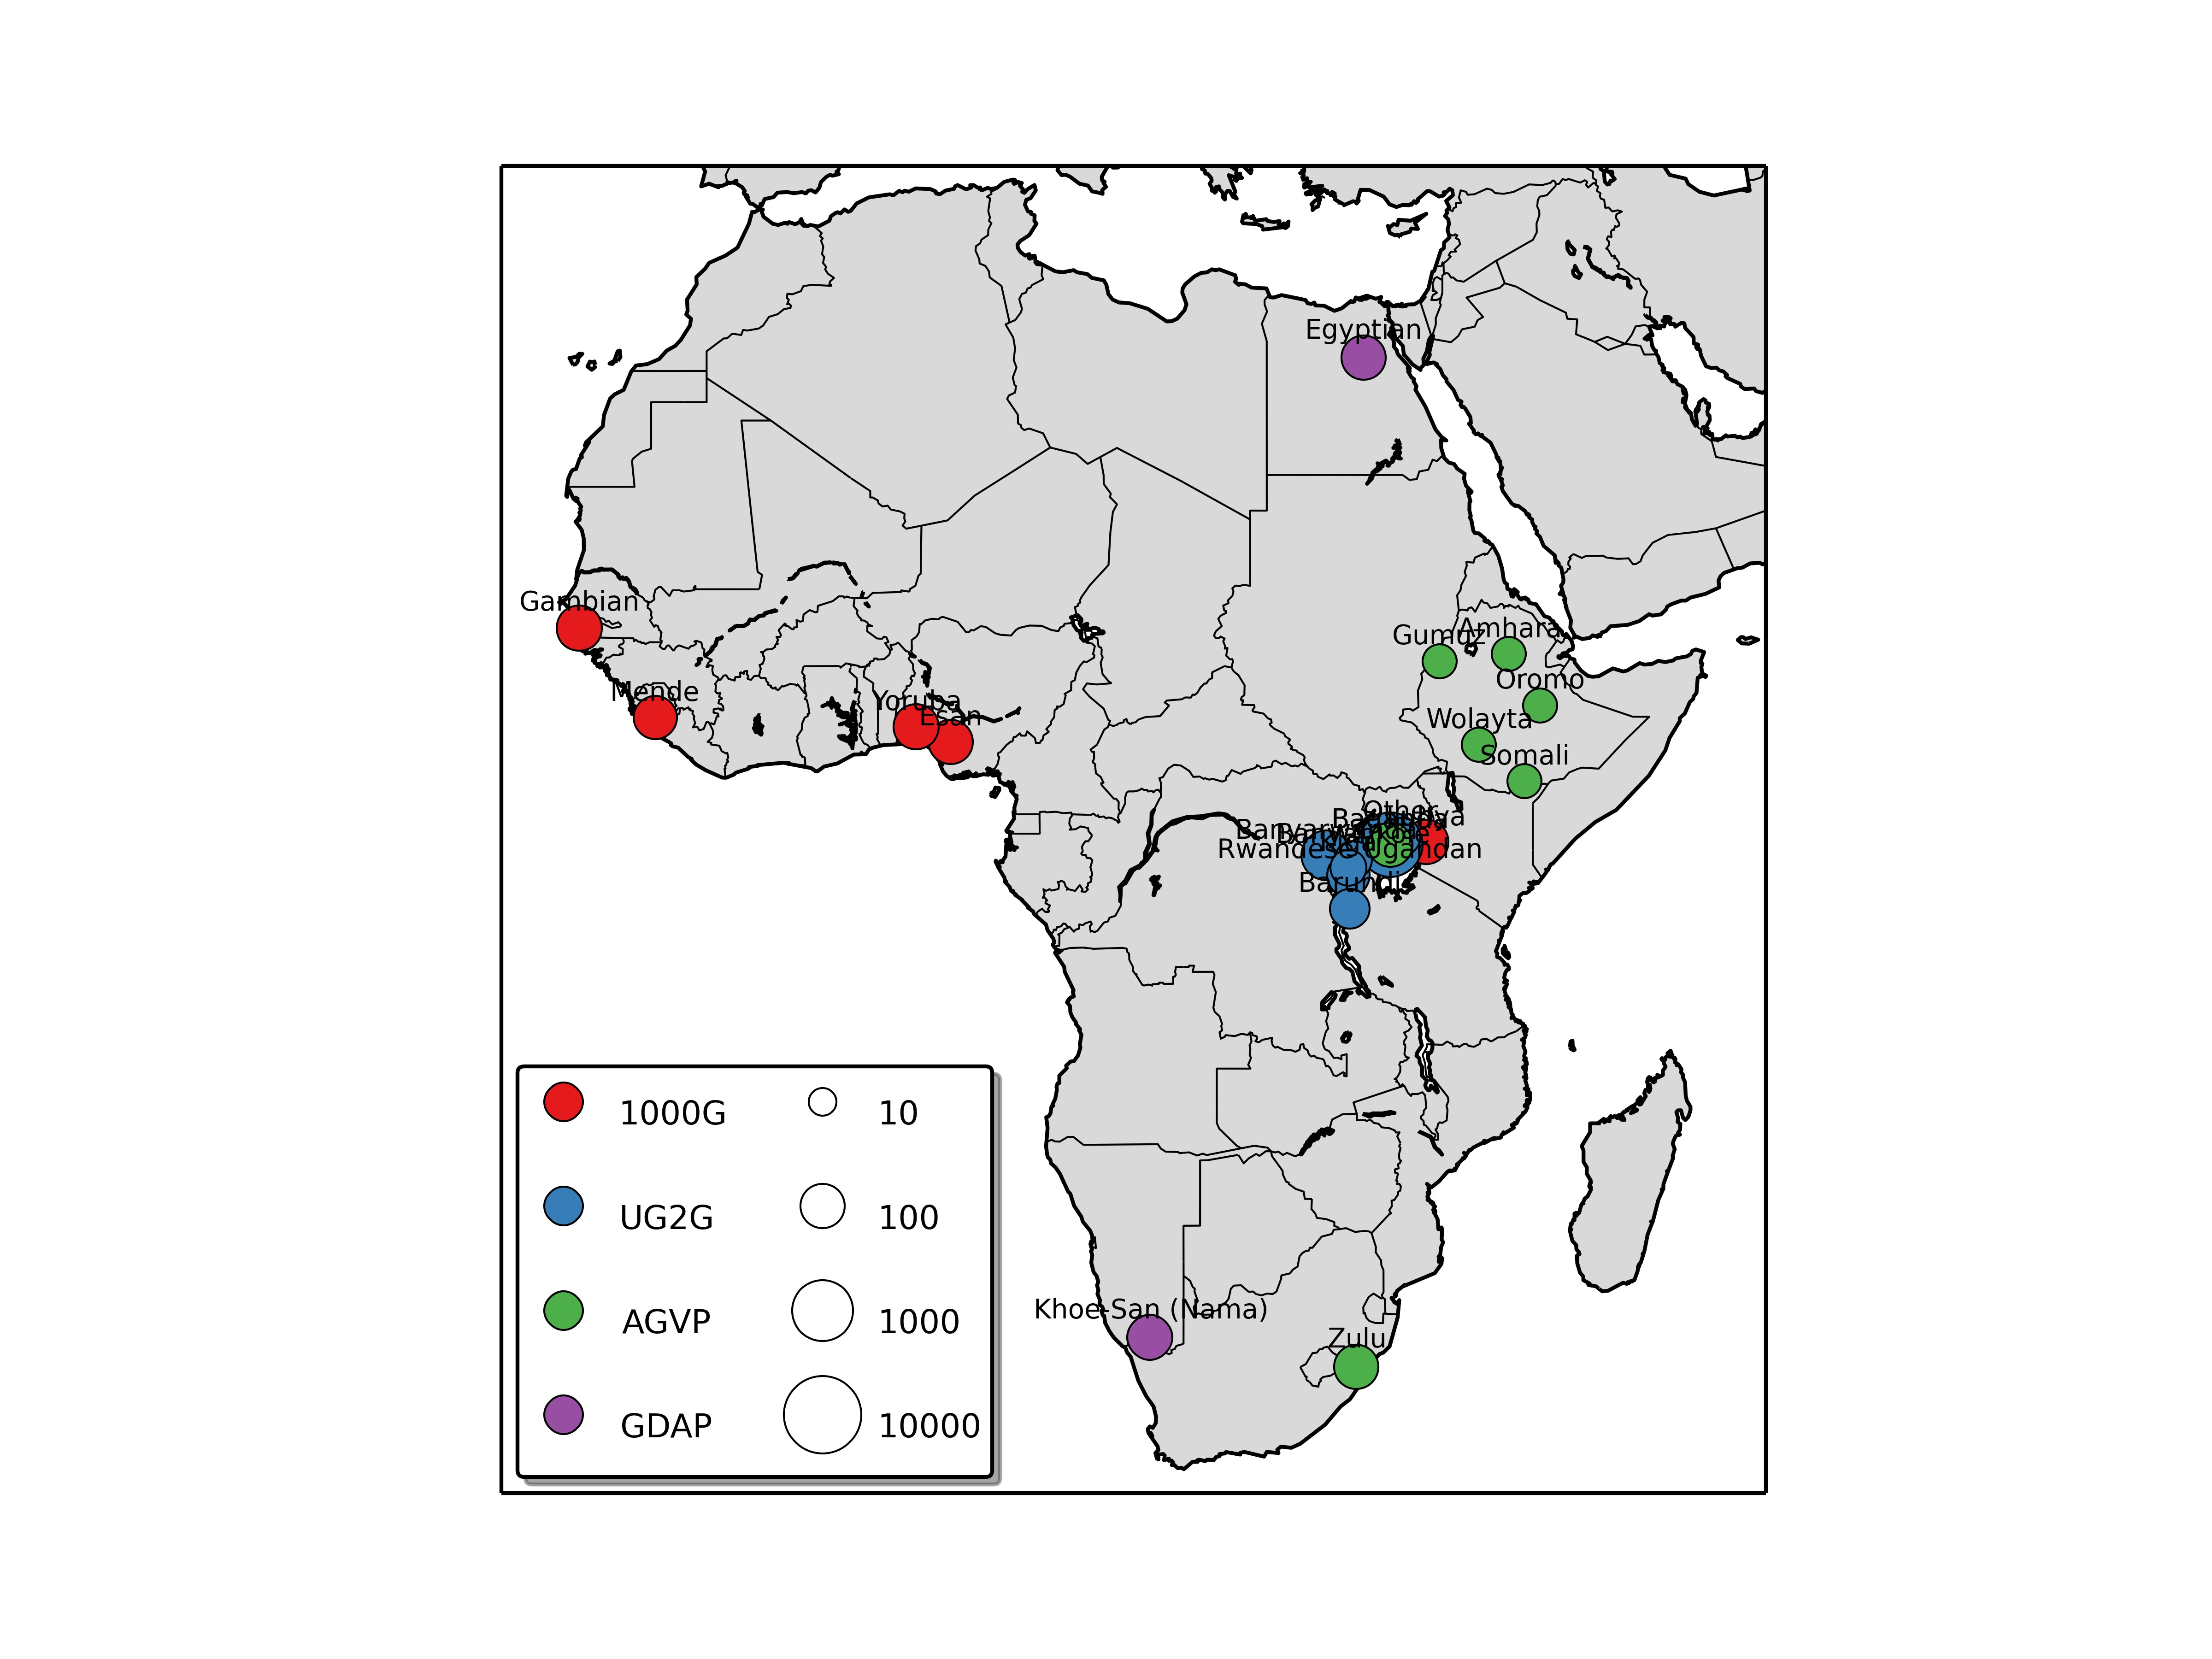
\includegraphics[width=1.0\linewidth]{Africa.jpg}
  \caption{African continent.}
\end{subfigure}%
\begin{subfigure}{.5\textwidth}
  \centering
  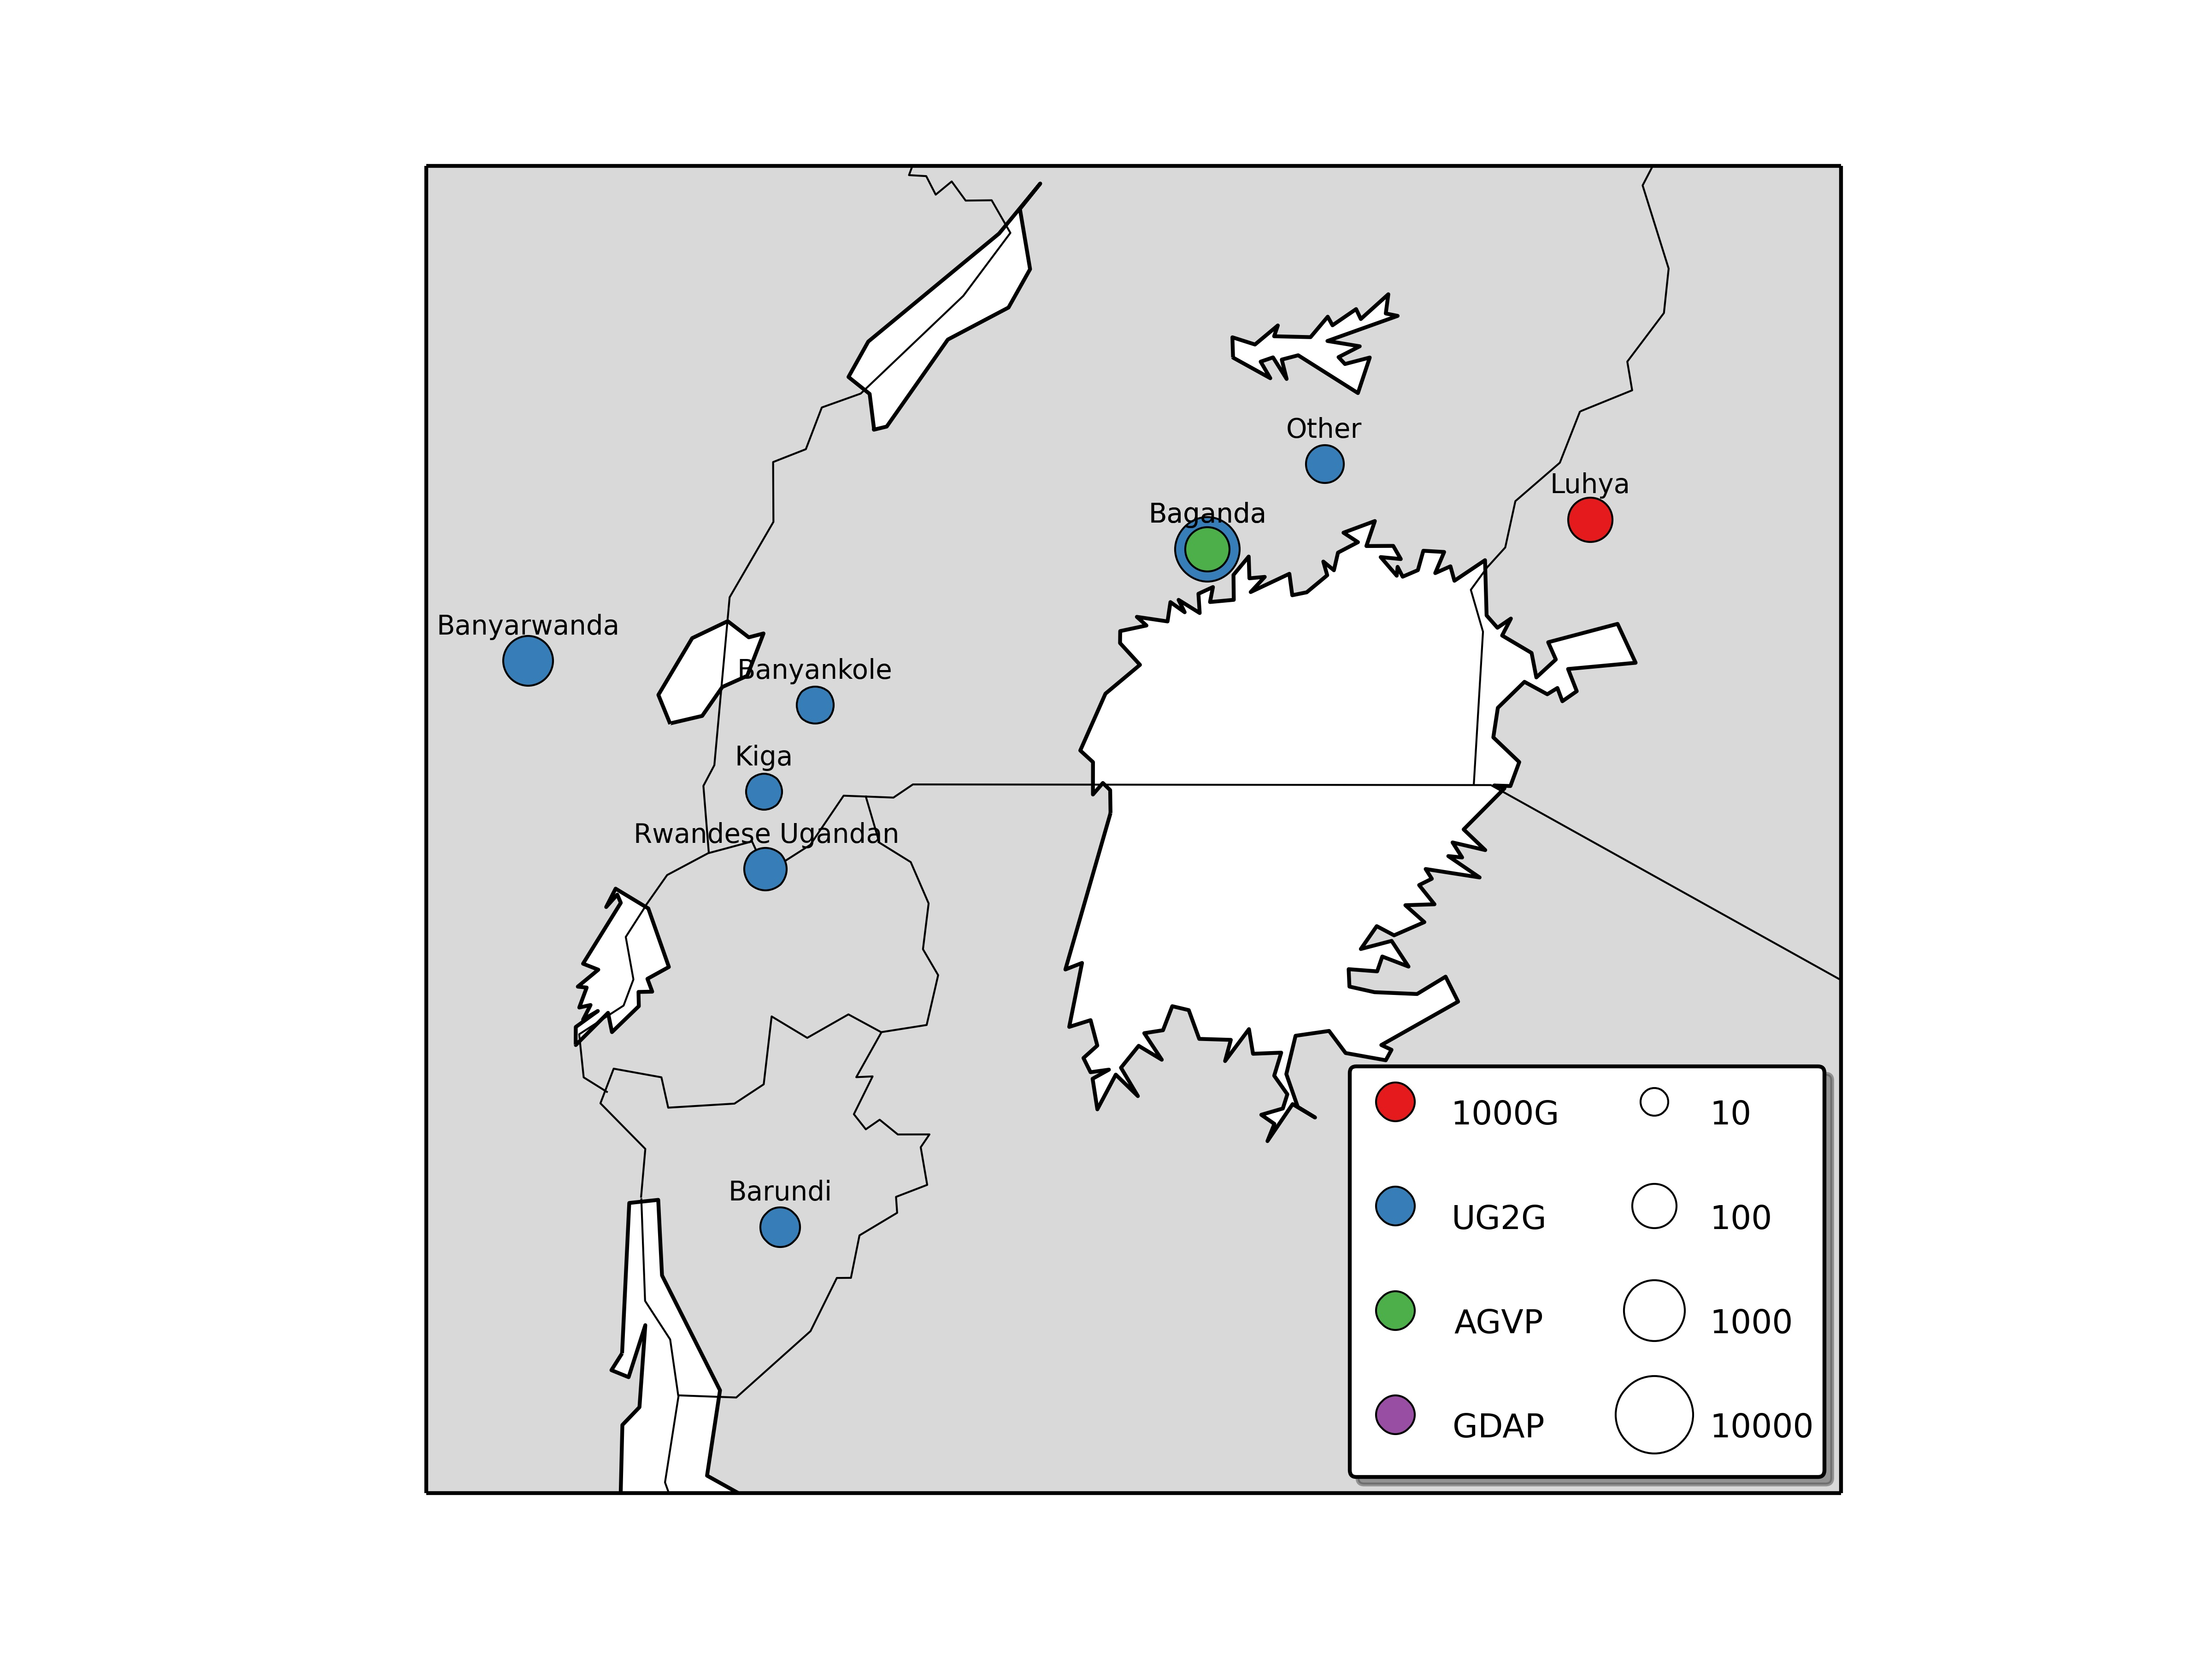
\includegraphics[width=1.0\linewidth]{Uganda.jpg}
  \caption{Southern Uganda south of the tripoint between Northern, Western and Eastern Africa.}
\end{subfigure}%
\caption{Maps showing sample location, sample count and sequencing depth of data to be included.}
\end{figure}

% I need to figure out how to avoid this table from exceeding the page width.
\begin{landscape}
\begin{longtable}{lllllll}
%\centering
\caption{Sample sets to be included in design of the African chip array}
\label{table:samples}
%\resizebox{\textwidth}{!}{%
%\begin{tabular}
\hline
Country & Ethnolinguistic group & No. & Seq depth & Source & Location & Size (TB) \\
\hline
\endhead % all the lines above this will be repeated on every page
Uganda & Baganda & 1567 & 4x & UG2G & WTSI & 40.4 \\
Uganda & Banyarwanda & 199 & 4x & UG2G & WTSI & 5.1 \\
Uganda & Rwandese Ugandan & 76 & 4x & UG2G & WTSI & 1.9 \\
Uganda & Barundi & 51 & 4x & UG2G & WTSI & 1.4 \\
Uganda & Banyankole & 36 & 4x & UG2G & WTSI & 0.93 \\
Uganda & Bakiga & 30 & 4x & UG2G & WTSI & 0.76 \\
Uganda & Other & 41 & 4x & UG2G & WTSI & 1.1 \\
Uganda & Baganda & 100 & 4x & AGVP & WTSI & 2.7 \\
South Africa & Zulu & 100 & 4x & AGVP & WTSI & 2.3 \\
Ethiopia & Amhara & 24 & 8x & AGVP & WTSI & 1.0 \\
Ethiopia & Gumuz & 24 & 8x & AGVP & WTSI & 1.0 \\
Ethiopia & Oromo & 24 & 8x & AGVP & WTSI & 1.0 \\
Ethiopia & Somali & 24 & 8x & AGVP & WTSI & 1.0 \\
Ethiopia & Wolayta & 24 & 8x & AGVP & WTSI & 1.0 \\
Egypt & Unspecified & 100 & 8x & GDAP & WTSI & 5.0 \\
South Africa & Khoe-San (Nama) & 104 & 4x & GDAP & WTSI & 3.6 \\
%Uganda & Baganda & 3 & 30x & GDAP & WTSI \\
%South Africa & Zulu & 2 & 30x & GDAP & WTSI \\
%South Africa & Khoe-San (Nama) & 3 & 30x & GDAP & WTSI \\
%Chad & Northern and Southern & 100 & 30x & GDAP & WTSI \\
%Kenya & Kalenjin & 100 & 30x & GDAP & WTSI \\
%Nigeria & Igbo & 100 & 30x & GDAP & WTSI \\
%Ghana & Ashanti & 100 & 30x & GDAP & WTSI \\
%Morocco & Moroccans & 100 & 30x & GDAP & WTSI \\
%Burkina Faso & Gouin, Kaboro, Turka & 100 & 30x & GDAP & WTSI \\
Gambia & Fula & 100 & 8x & MalariaGEN & ENA \\
Nigeria & Esan & 99 & 4x & 1000G & 1000G \\
Gambia & Gambian, Western div & 113 & 4x & 1000G & 1000G \\
Kenya & Luhya in Webuye & 116 & 4x & 1000G & 1000G \\
Sierra Leone & Mende & 85 & 4x & 1000G & 1000G \\
Nigeria & Yoruba in Ibadan & 116 & 4x & 1000G & 1000G \\
Gambia & Gambian & 2 & 30x & 1000G & Simons Foundation \\
Nigeria & Esan & 2 & 30x & 1000G & Simons Foundation \\
Sierra Leone & Mende & 2 & 30x & 1000G & Simons Foundation \\
Kenya & Luhya & 2 & 30x & Coriell & Simons Foundation \\
Kenya & Masai & 2 & 30x & Coriell & Simons Foundation \\
Kenya & Luo & 2 & 30x & Geoge Ayodo & Simons Foundation \\
Kenya & Somali & 1 & 30x & Geoge Ayodo & Simons Foundation \\
Algeria & Mozabite & 8 & 8x & HGDP/Martin et al 2014 & NCBI-SRA \\
DRC & Mbuti & 8 & 7x & HGDP/Martin et al 2014 & NCBI-SRA \\
Namibia & San (Ju-hoan) & 6 & 10x & HGDP/Martin et al 2014 & NCBI-SRA \\
Algeria & Mozabite & 2 & 30x & HGDP/Reich+Tyler-Smith & Simons Foundation and WTSI \\
%South Africa & Bantu (Tswana, Herero, Pedi, Sotho, Ovambo, Zulu) & 8 & 30x & HGDP/Reich+Tyler-Smith & Simons Foundation and WTSI \\
South Africa & \begin{tabular}[b]{@{}l@{}}Bantu\\(Tswana, Herero, Pedi, Sotho, Ovambo, Zulu)\end{tabular} & 8 & 30x & HGDP/Reich+Tyler-Smith & Simons Foundation and WTSI \\
Kenya & Bantu & 11 & 30x & HGDP/Reich+Tyler-Smith & Simons Foundation and WTSI \\
CAR & Biaka Pygmy & 23 & 30x & HGDP/Reich+Tyler-Smith & Simons Foundation and WTSI \\
Senegal & Mandenka & 22 & 30x & HGDP/Reich+Tyler-Smith & Simons Foundation and WTSI \\
DRC & Mbuti Pygmy & 12 & 30x & HGDP/Reich+Tyler-Smith & Simons Foundation and WTSI \\
Namibia & San (Ju-hoan) & 6 & 30x & HGDP/Reich+Tyler-Smith & Simons Foundation and WTSI \\
Nigeria & Yoruba & 21 & 30x & HGDP/Reich+Tyler-Smith & Simons Foundation and WTSI \\
South Africa & Khomani & 2 & 4x/9x & Kidd et al 2014 & NCBI-SRA \\
South Africa & Khomani & 2 & 30x & Brenna Henn & Simons Foundation \\
Sudan & Dinka & 3 & 30x & Michael Hammer & Simons Foundation \\
Namibia & Khoisan & 1 & 10x & Schuster et al 2009 & NCBI-SRA \\
South Africa & Xhosa/Tswana & 1 & 30x & Schuster et al 2009 & NCBI-SRA \\
North Africa & Arab-/Berber-speaking groups & ?? & 20x & Private (David Comas) &  \\
Morocco & Saharawi & 2 & 30x & David Comas & Simons Foundation \\
South Africa & Mixed (Cape Coloured) & 8 & 30x & SAHGP &  \\
South Africa & Sotho & 8 & 30x & SAHGP &  \\
South Africa & Xhosa & 8 & 30x & SAHGP &  \\
Total* &  & 3936 &  &  & 
%\end{tabular}
}
\end{longtable}
\end{landscape}
\section{Generation of haplotypes from raw reads}
Given the need to include large sample sizes from diverse populations for such a resource for development of an African chip, curation of data will involve generation of homogenised data from different datasets, including publicly available data as outlined in Table 1. Given the heterogeneity in sequencing and coverage among datasets (Table 1), these will need to be processed in subsets, and then merged to generate a complete panel of all variants. 

Publicly available curated data from the \href{http://www.1000genomes.org}{1000 Genomes project (1000G)}
%and the \href{http://www.simonsfoundation.org/}{Simon’s Foundation}
will be used as such. For datasets that are sequenced in house, consistent methods will be used for curation.

\subsection{Alignment and preprocessing of reads}
Following generation of raw reads mapping will be carried out to the human reference genome (GRCh37) using the BWA-MEM algorithm of the BWA software package, which is suitable for Illumina reads longer than 70bp.\cite{2013arXiv1303.3997L} Optical and PCR duplicate reads will be marked with Picard MarkDuplicates on a lanelet level. The reads will be sorted by coordinate with samtools sort. The lanelets will be merged to a library level with Picard MergeSamFiles, and duplicate reads will be marked on a library level. The BAMs will be merged to a sample level and then sample level bam improvement will be carried out using GATKv2.8+. This process will consist of a per-sample realignment of reads around known and discovered indels with GATK RealignerTargetCreator and IndelRealigner in addition to base quality score recalibration (BQSR) with GATK BaseRecalibrator and PrintReads.

\subsection{Quality control prior to variant calling}
We require that the percentage of aligned reads is 90\% or greater, which we check with samtools flagstat. Prior to variant calling we check for contamination and sample mix up with VerifyBamID and require that the calculated FREEMIX is less than 0.05.
%Prior to variant calling we check the gender of the samples with GATK3.3+ DepthOfCoverage and require that the ratio between the non-PAR X and Y coverage is less than 2 and greater than 5 for males and females, respectively.

\subsection{Evaluation of variant calling software packages}
Prior to variant calling across all datasets we determined the best variant calling and filtering method for SNPs, short indels and SVs for African low coverage data. Specifically variant calling was carried out for chromosome 20 of 1986 Ugandan low coverage samples using several algorithms; samtools, GATK HaplotypeCaller (HC) and GATK UnifiedGenotyper (UG). To make assesment of the sensitivity and specificity for each variant caller possible calling was carried out with a sample sequenced at similar coverage from the \href{http://genomeinabottle.org}{Genome in a Bottle (GiaB)} highly curated set. PCR-free reads will be used for the validation sample to avoid PCR artefacts. The GiaB sample (NA12878) represents a CEU sample from a 12 person pedigree in 1000G that has gone through extensive curation and validation of variants.\cite{Zook2014} The software with the greatest area under the ROC (sensitivity, 1-specificity) curve will be used for calling SNPs from the low coverage data.
%These callers may be different for SNPs, short indels and SVs. Calling and filtering of SNPs, indels and long deletions will be carried out separately using the chosen algorithm(s), with filtering thresholds chosen for SNPs and short indels based on the sensitivity and specificity on the platinum genomes sample.

EDIT!!!!

In order to explore the sensitivity and specificity of variant callers when applied to low coverage datasets, we carried out an evaluation with 1,986 samples from Uganda sequenced at 4x average coverage with Illumina HiSeq 2000. The down-sampled GiaB sample\cite{Zook2014} (6x) was included in the called set for validation. We calculated the sensitivity and specificity of calls relative to the highly curated variant sites for the NA12878 sample, to identify the caller with greatest area under ROC curve at different filtering thresholds (Figure 3). We used two different filtering thresholds for this analysis: the SNP quality metric (QUAL), and the VQSLOD score obtained using the VQSR model implemented by GATK for different callers. With this evaluation, we show that UnifiedGenotyper3.2 shows the best area under ROC curve with the lowest FDR for a given sensitivity for SNPs and indels (Figure \ref{fig:roc}). All callers, however produce very low sensitivity and high FDRs for indel calls (Figure \ref{fig:roc_indels}). It is likely that the sensitivity and specificity of calls will improve with genotype refinement, particularly when carried out along with high coverage data from X10 sequencing. Variant Quality score recalibration (VQSR) based filtering approaches seem to perform better than filtering only on variant quality for most calls. However, further exploration of filtering approaches for indel calls is needed, including appropriate normalisation of model training sets, as this could potentially improve the sensitivity for a given FDR. Additionally, a new release of HaplotypeCaller corrects issues with previous releases, potentially greatly improving the sensitivity for SNPs and indels. A comparison of these callers with consistent filtering methods will inform the best method to use for calling SNPs and indels within low coverage (4x) data. Choosing appropriate callers and filtering methods is crucial maximising variant discovery while maintaining low false discovery on the panel curated for the development of the chip array.

\begin{figure}[h]
\captionsetup{width=0.8\textwidth}
\caption{An evaluation of calling algorithms for SNPs and indels in low coverage data. The figure depicts a comparison of various calling algorithms using different filters for calling SNPs (left) and indels (right) in low coverage data. The x axis represents the false discovery rate (FDR), which is defined as the proportion of calls produced by a given algorithm that are false positives at a given filtering threshold. The y axis represents the true positive rate or the sensitivity, which is the proportion of all true calls in the GiaB sample that are captured by a given algorithm for a given filtering threshold. The curves are generated by varying filtering thresholds for each algorithm. UG: UnifiedGenotyper; FB: FreeBayes; HC: HaplotypeCaller; QUAL: Phred-scaled quality score; VQSLOD: Variant Quality Recalibration scores; NIST: National Institute of Standards and Technology.}
\label{fig:roc}
\centering
    \begin{subfigure}[b]{0.45\textwidth}
        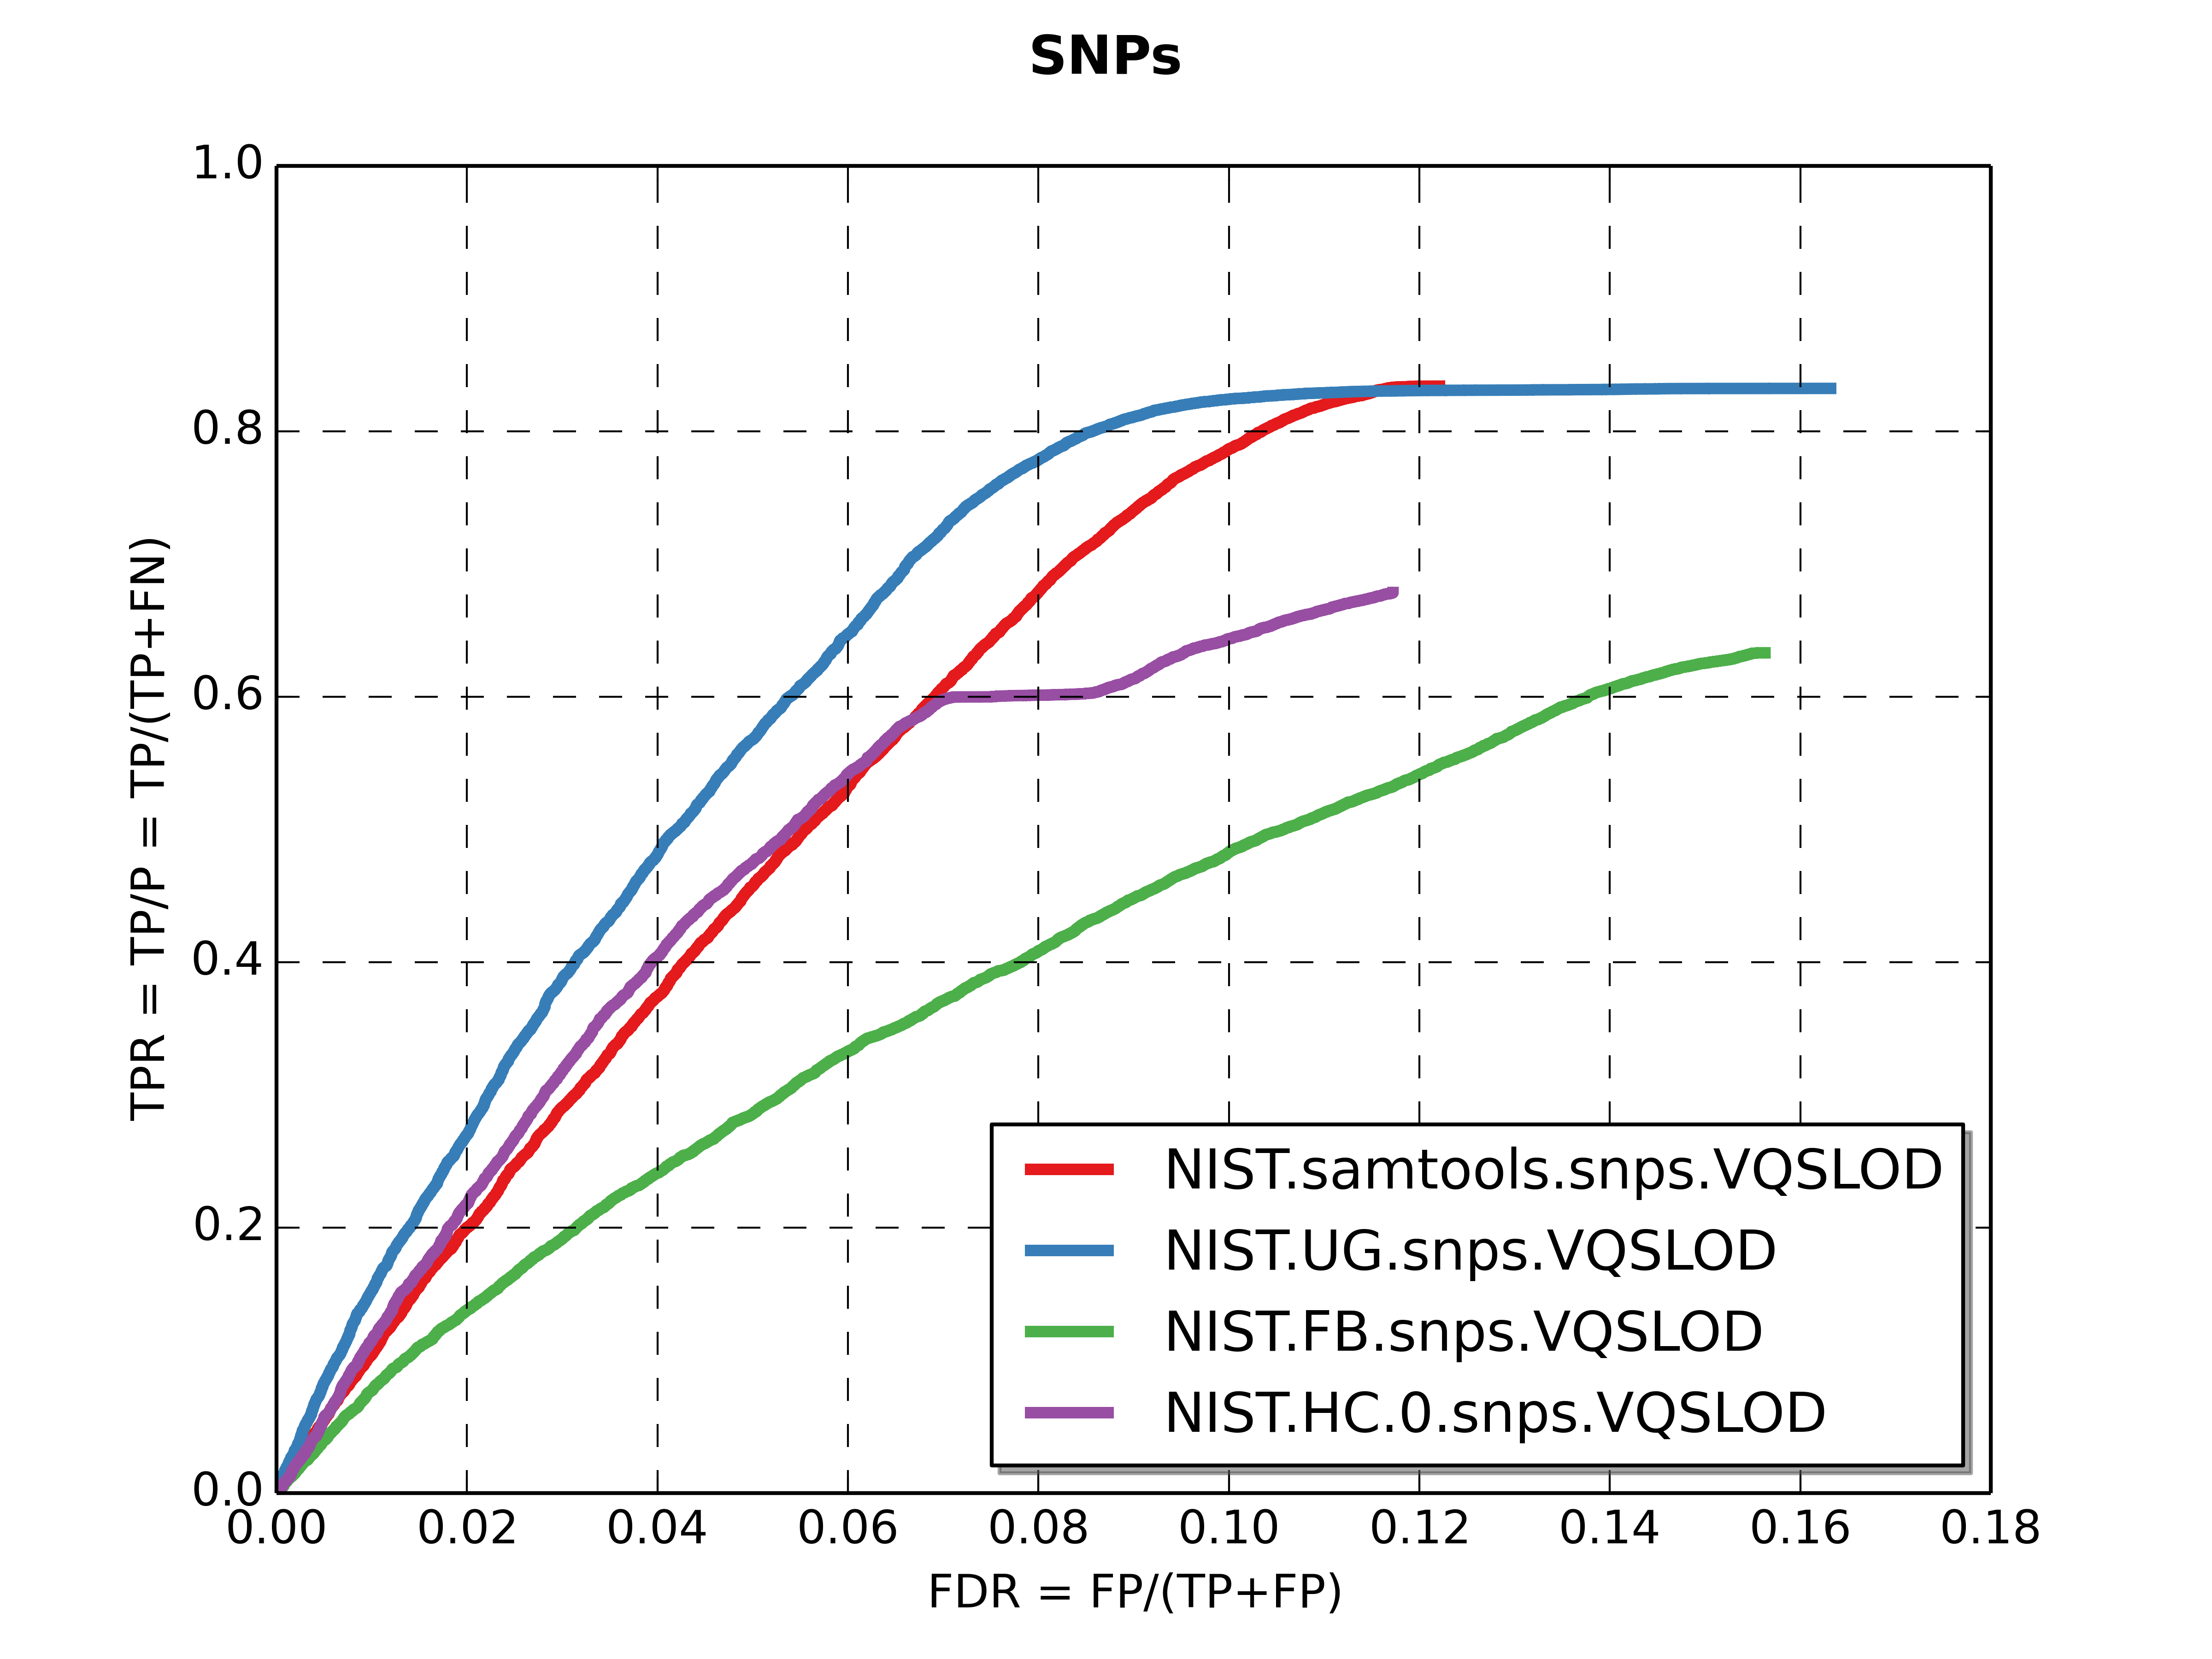
\includegraphics[width=\textwidth]{FDR_snps}
        \caption{SNPs}
        \label{fig:roc_snps}
    \end{subfigure}%
    \begin{subfigure}[b]{0.45\textwidth}
        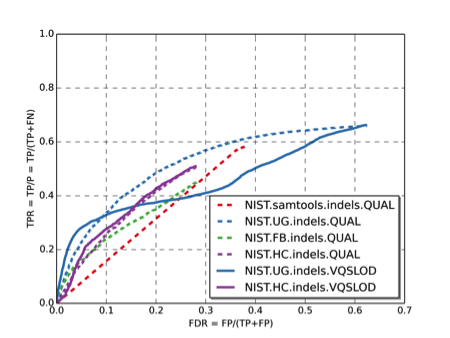
\includegraphics[width=\textwidth]{FDR_indels}
        \caption{Indels}
        \label{fig:roc_indels}
    \end{subfigure}%
\end{figure}

For high coverage data, we evaluated the NA12878 sample alone re-sequenced on the X-10 pipeline with the highly curated set of variants produced by GiaB.1 We showed that the X-10 and the new pipeline used with it produced high quality data that when normalised showed a high degree of sensitivity versus the GiaB reference set and a low false discovery rate (Table \ref{table:highcoverage}). When the Illumina 50x Platinum set, sequenced on the Illumina Hiseq 2000 platform was reprocessed through the same pipeline it produced similarly high results, though the INDEL sensitivity and false discovery rate were slightly better. We believe this may be because of the higher coverage and PCR free library preparation used in the creation of this sequence.

\begin{table}[h]
\centering
%\resizebox{\textwidth}{!}{%
\begin{tabular}{l|lrrrrr}
\rowcolor[HTML]{333333} 
{\color[HTML]{FFFFFF} Sample} & {\color[HTML]{FFFFFF} Type} & {\color[HTML]{FFFFFF} TP} & {\color[HTML]{FFFFFF} FP} & {\color[HTML]{FFFFFF} FN} & {\color[HTML]{FFFFFF} Sensitivity} & {\color[HTML]{FFFFFF} FDR} \\
 & \cellcolor[HTML]{C0C0C0}SNP & \cellcolor[HTML]{C0C0C0}2914294 & \cellcolor[HTML]{C0C0C0}28213 & \cellcolor[HTML]{C0C0C0}10266 & \cellcolor[HTML]{C0C0C0}0.9965 & \cellcolor[HTML]{C0C0C0}0.0096 \\
\multirow{-2}{*}{Replicate 1} & INDEL & 413639 & 23145 & 34743 & 0.9255 & 0.0530 \\
 & \cellcolor[HTML]{C0C0C0}SNP & \cellcolor[HTML]{C0C0C0}2908260 & \cellcolor[HTML]{C0C0C0}26311 & \cellcolor[HTML]{C0C0C0}14452 & \cellcolor[HTML]{C0C0C0}0.9951 & \cellcolor[HTML]{C0C0C0}0.0090 \\
\multirow{-2}{*}{Replicate 2} & INDEL & 393431 & 24110 & 52542 & 0.8822 & 0.0577 \\
 & \cellcolor[HTML]{C0C0C0}SNP & \cellcolor[HTML]{C0C0C0}2917290 & \cellcolor[HTML]{C0C0C0}21400 & \cellcolor[HTML]{C0C0C0}9844 & \cellcolor[HTML]{C0C0C0}0.9966 & \cellcolor[HTML]{C0C0C0}0.0073 \\
\multirow{-2}{*}{Platinum} & INDEL & 437875 & 8802 & 2297 & 0.9948 & 0.0197
\end{tabular}
%}
\caption{Intersect of NA12878 samples with GiaB reference calls version 0.2.}
\label{table:FDRhigh}
\end{table}

\subsection{Variant calling}
After deciding on the best software we will carry out variant calling.
%Datasets generated with unique Illumina chemistry, and those with different coverages will need to be called in separate subsets. GATK3.3+ UnifiedGenotyper (UG) and GATK3.3+ HaplotypeCaller (HC) will be used for calling SNPs from low and high coverage data, respectively. Multiple samples will be called simultaneously with UnifiedGenotyper, whereas HaplotypeCaller will be applied to individual samples in GVCF mode and subsequently joint genotyping will be carried out with GenotypeGVCFs. For compatibility reasons it is important that the same versions of HaplotypeCaller and GenotypeGVCFs are used.
%http://gatkforums.broadinstitute.org/discussion/5051/are-gatk-versions-3-compatible
During variant calling UG by default downsamples each sample randomly to a maximum coverage of 250 (--downsampling\_type BY\_SAMPLE and --downsample\_to\_coverage 250). We will use the default minimum base quality for UG, which is currently 17 (--min\_base\_quality\_score 17). %10 for HC
At each site we don't call more than the 6 best alternate alleles (--max\_alternate\_alleles 6).
For low coverage data we use calling and emission thresholds (--standard\_min\_confidence\_threshold\_for\_calling and --standard\_min\_confidence\_threshold\_for\_emitting) of 10 and 4 if the sample count is greater than and less than 100, respectively.
%For high coverage data we use thresholds of 30 in accordance with GATK best practices.
%Indels will be called with a plethora of software packages (see the next section).

%If pedigree information is available, then this will be used by UnifiedGenotyper %and GenotypeGVCFs
%in calculation of the InbreedingCoeff annotation, which is used for subsequent variant filtering. Pedigree information will also be used for refinement and phasing. Incomplete pedigrees will be inferred from IBD matrices for sequenced and non-sequenced samples in each cohort.

%\subsubsection{Calling of short indels and structural variants}
With UG we will only make a call in the low coverage data, if the number of consensus indels exceeds a threshold of 5 (--min\_indel\_count\_for\_genotyping 5), which is the default value and the value used for phase 1 of 1000G.
%1000G low coverage indel calling by the Broad - "if a candidate indel allele was present in at least 5 reads at a site, it would be passed over to the next step for genotyping, or otherwise it was excluded."
We furthermore use PINDEL, GINDEL, Dindel, samtools, MATE-CLEVER and SOAPdenovo to call indels shorter than 100bp and deletions longer than 100bp. Breakdancer is used to identify structural variants (SVs) in trios. GenomeSTRiP is used for discovery of deletions. We will use best practices of each method to filter variants prior to creating a consensus set. For Pindel for example it will be a requirement that an indel appear in more than 3 samples and with more than 10 supporting reads in total among all samples.
%GoNL Indels (1-20bp) "GATK UG and at least one other algorithm"
%GoNL Deletions (20-100bp) "more than one method" "at least 3 families and transmitted to at least 1 child"
%GoNL Deletions (>100bp) "at least two algorithms" "at least 3 families and transmitted to at least 1 child"

We remove indels with the maximum number of alternate alleles.
%1000G called indels as biallelic.
Similar to 1000G we will remove protein-coding frameshift indels exclusive to low coverage samples and do post-hoc filtering of short indels with a support vector machine (SVM) or random forest (RF) machine learning approach and by applying a MAF threshold of 0.5\%. The latter machine learning method has been used successfully at the Broad Institute. One could classify indels by:
\begin{enumerate}
\item length (continuous or classified)
\item type (homopolymer run (HR) with runs of 6 or more identical nucleotides, tandem repeat (TR))
\item frameshift/nonframeshift in coding regions
\item tandem repeat length (dinucleotide repeat, trinucleotide repeat, STR/microsatellite (2-5/6/9), minisatellite (10-60)
%INSERTION-DELETION VARIANTS IN 179 HUMAN GENOMES - Table 3 - Characteristics of indels
\item HR insertion (more likely), HR deletion (less likely)
\item tandem repeat type (CG, non-CG)
\item SNP at same site, no SNP at same site
\item biallelic, multialleic
\item inside/outside RepeatMasker regions
\item P site / non-P site; i.e. the reference base not N, depth not less than half of average, depth not twice of average, less than 20\% of reads at position have MQ of 0, base not covered. Calculate averages for the autosomes and the X chromosome independently.
\item allele balance
\item strand bias
\item mapping quality
\item number of supporting non-reference reads
\item distance to nearby indels
\item cytoband: gneg, gpos25, gpos50, gpos75, gpos100, acen, gvar
\end{enumerate}

The NIST NA12878 truth set currently does not hold information on structural variants (SVs). We therefore carry out calling of SVs with multiple callers, apply default calling thresholds and use a consensus dataset as the final SV dataset.

Other variant callers to consider are listed in the table below.
\input{tables/INDELcallers}

\subsubsection{Calling of chromosomes X and Y}
The X chromosome will be called jointly for males and females with the same ploidy, because the memory and CPU use of UG otherwise grows intensely. Likewise the pseudoautosomal regions (PARs) 1 and 2 on the X chromosome will be called like the autosomes; i.e. jointly for males and females with all samples treated as diploid. The Y chromosome will also be treated as diploid due to the UG memory and CPU issue, when doing haploid variant calling, but variant calling will only be carried out for males. The PARs on the Y chromosome are masked in the reference sequence and not subject to calling. An excessive number of heterezogyous calls of haploid genotypes can be utilized for a QC step of sites and samples; thresholds to be decided.
%The mitochondrial variants will be called with GATK, VarScan2\cite{Koboldt2012} and MitoSeek and the union set recalled and annotated with GATK prior to filtering. VarScan is chosen, because it performs well at extreme read depths.\cite{Stead2013} MitoSeek is a software package dedicated to calling variants from mtDNA reads. When calling with GATK the ploidy will be set to the mean coverage in the MT contig divided by the mean coverage in the somatic chromosomes.
%http://gatkforums.broadinstitute.org/discussion/1214/can-i-use-gatk-on-non-diploid-organisms
%GoNL - "Consensus sequences were called by GATK."

%\begin{table}[h]
\centering
\begin{tabular}{l|l|l|}
\cline{2-3}
\rowcolor[HTML]{FFFFFF} 
                          & Male & Female \\ \hline
\multicolumn{1}{|l|}{X}   & 1    & 2      \\ \hline
\multicolumn{1}{|l|}{Y}   & 1    & N/A    \\ \hline
\multicolumn{1}{|l|}{PAR} & 2    & 2      \\ \hline 
\end{tabular}
\caption{Ploidies used for calling variants on the sex chromosomes.}
\label{table:XYcalling}
\end{table}


\subsection{Variant Filtering}
Filtering will be carried out with GATK3.3+ VariantRecalibrator, which does variant quality score recalibration (VQSR). VQSR will be applied simultaneously across the autosomes and the sex chromosomes. GATK best practices will be used for filtering SNPs.
%http://gatkforums.broadinstitute.org/discussion/1259/which-training-sets-arguments-should-i-use-for-running-vqsr
We will use HapMap III and 1000G phase 1 Omni2.5 sites as truth and training sets (prior probabilities of 15 and 12). High confidence 1000G phase 1 SNPs will be used as an additional training set (prior 10). This dataset does not contain Y chromosome variants. %For indels we will use the Mills and Devine and 1000G gold standard as a truth and training set (prior 12). In both cases
dbSNP138 or newer will act as a set of known sites.
To build our VQSR Gaussian mixture model we use annotations at each site related to coverage (QD=QualByDepth and DP), strand bias (FS=FisherStrand, SOR=StrandOddsRatio), mapping quality (MQ, MQRankSum, ReadPosRankSum).
%For indels we use the same annotations, except for MQ being left out.
DP is the approximate read depth after filtering reads with poor mapping quality and bad mates. QD is the variant confidence normalized by the unfiltered depth for the variant allele. FS is a Phred-scaled p-value using Fisher's exact test to detect strand bias. SOR is the odds ratio of a 2x2 contingency table (rows and columns are positive/negative strand and reference/alternate allele) to detect strand bias. MQ is the RMS of the mapping qualities, which serves an an average across reads and samples. MQRankSum is the Z-score from a Wilcoxon rank sum test of alternate vs. reference mapping qualities. ReadPosRankSum is the Z-score from a Wilcoxon rank sum test of alternate vs. reference read position biases.
%When not doing variant calling with HaplotypeCaller we
We will also use the annotation HaplotypeScore, which is a statistical measure of more than 2 haplotypes being present at the same site for a sample.

The NA12878 sample will be included at an appropriate coverage, when doing variant calling. PCR-free reads will be used for the validation sample to avoid PCR artefacts. The inclusion of NA12878 allows for selection of a filtering threshold, which yields a good balance between sensitivity and specificity after filtering. Specifically ROC curves will be generated for sample NA12878, for which highly curated SNPs
%and short INDELs
are available for chromosomes 1-22 and X. The ROC curves will be sorted by the variant quality score log odds ratios calculated by VariantRecalibrator.
%For structural variants we will use PacBio 54x NA12878 WGS data as a truth set. %ftp://ftp.1000genomes.ebi.ac.uk/vol1/ftp/technical/working/20131209_na12878_pacbio/si/

%For cohorts with 10 or more founder samples the InbreedingCoeff annotation will also be used. It is a likelihood-based Hardy-Weinberg test for the inbreeding among samples. It will be tested by generation of additional ROC curves, whether the inclusion of the InbreedingCoeff annotation worsens the ability to do VQSR correctly, when there are many related samples. Whenever available pedigree information will be used during variant calling to assist in the calculation of the InbreedingCoeff annotation.

%We apply the filtering by doing a binary heap merge of unfiltered variants to 1) allow two VQSR processes to run simultaneously; i.e. one for SNPs and one for indels and to 2) avoid lexicographical sorting of already numerically sorted files (i.e. VCF and recal files are sorted numerically by genomic coordinate). Alternatively one can run GATK VariantRecalibrator and ApplyRecalibration in sequence twice, which is twice as slow. Furthermore the heap merge only requires a line from the SNP .recal file, the INDEL .recal file and the VCF file to be held in memory at once.
%The excludemarkers option of the current release of Beagle4 cannot be used to apply the filtering, because 1) UG emits two separate VCF records for SNPs and indels at the same site and 2) the excludemarkers option of Beagle4 only allows one to specify variants by rsID or genomic coordinate. The excludemarkers option would otherwise save disk space and time.

Unlike 1000G and GoNL we will not filter out multiallelic variants, because we don't find them to be of lower quality than biallelic SNPs and because there is a greater probability of these appearing across thousands of samples from multiple populations from the African continent than in hundreds of samples from one European country. For example 1 in every ~50 SNP in ~2000 Ugandan samples sequenced to a depth of 4x is multiallelic.
%They probably did this, because Beagle3 didn't support multiallelic variants...

\subsection{Merging of Datasets}
Following curation of individual datasets, these will need to be merged to homogenise variant calls across all data, and generate a non-sparse matrix of variant calls, where the union of variants across all samples is available for each population. This process is similar to the merger of reference panels by imputation (Figure \ref{fig:merging_reference_panels}), which could have been used, if raw reads had not been available for all populations. In order to fill the sparse matrix a union set of calls will be generated for variants that have passed filtering in each dataset (Figure \ref{fig:calling}). Prior to merging we recode any haploid male genotypes (non-PAR X and Y) to homozygous diploid genotypes if necessary. %Prior to merging 1) indels will be left aligned (e.g. bcftools norm) and 2) SNPs and indels called in low coverage data by UnifiedGenotyper will be merged into single records with bcftools (bcftools norm -m +any).
%and 3) variants called from reads aligned to build 38 will be lifted over to build 37 (liftOver). %http://hgdownload.soe.ucsc.edu/admin/exe/linux.x86_64/liftOver
Variants will be merged across cohorts (GATK CombineVariants --minimalVCF or bcftools merge | bcftools view -G). These sites will then be recalled in each dataset to generate genotype likelihoods at these sites. Sample NA12878 will not be part of the recalling and NA12878 singletons will not be called.
%Where necessary the union set of sites will be lifted over to build 38 prior to recalling and the recalled variants will then be lifted back over to build 37.
UG (--genotyping\_mode GENOTYPE\_GIVEN\_ALLELES and --output\_mode EMIT\_ALL\_SITES) will be used for recalling low coverage data.
%http://gatkforums.broadinstitute.org/discussion/4936/not-all-sites-emitted-with-genotype-given-alleles
The maximum number of allowed alternate alleles will be increased from the default 6 by multiplication with the number of original cohorts to allow all true variants to be called. Although it should only be necessary for HaplotypeCaller, interval padding will be added to ensure all known sites are called (--interval\_padding 100).
%http://gatkforums.broadinstitute.org/discussion/comment/18353
Following this, genotype refinement will be carried out.

\begin{figure}[!htbp]
\centering
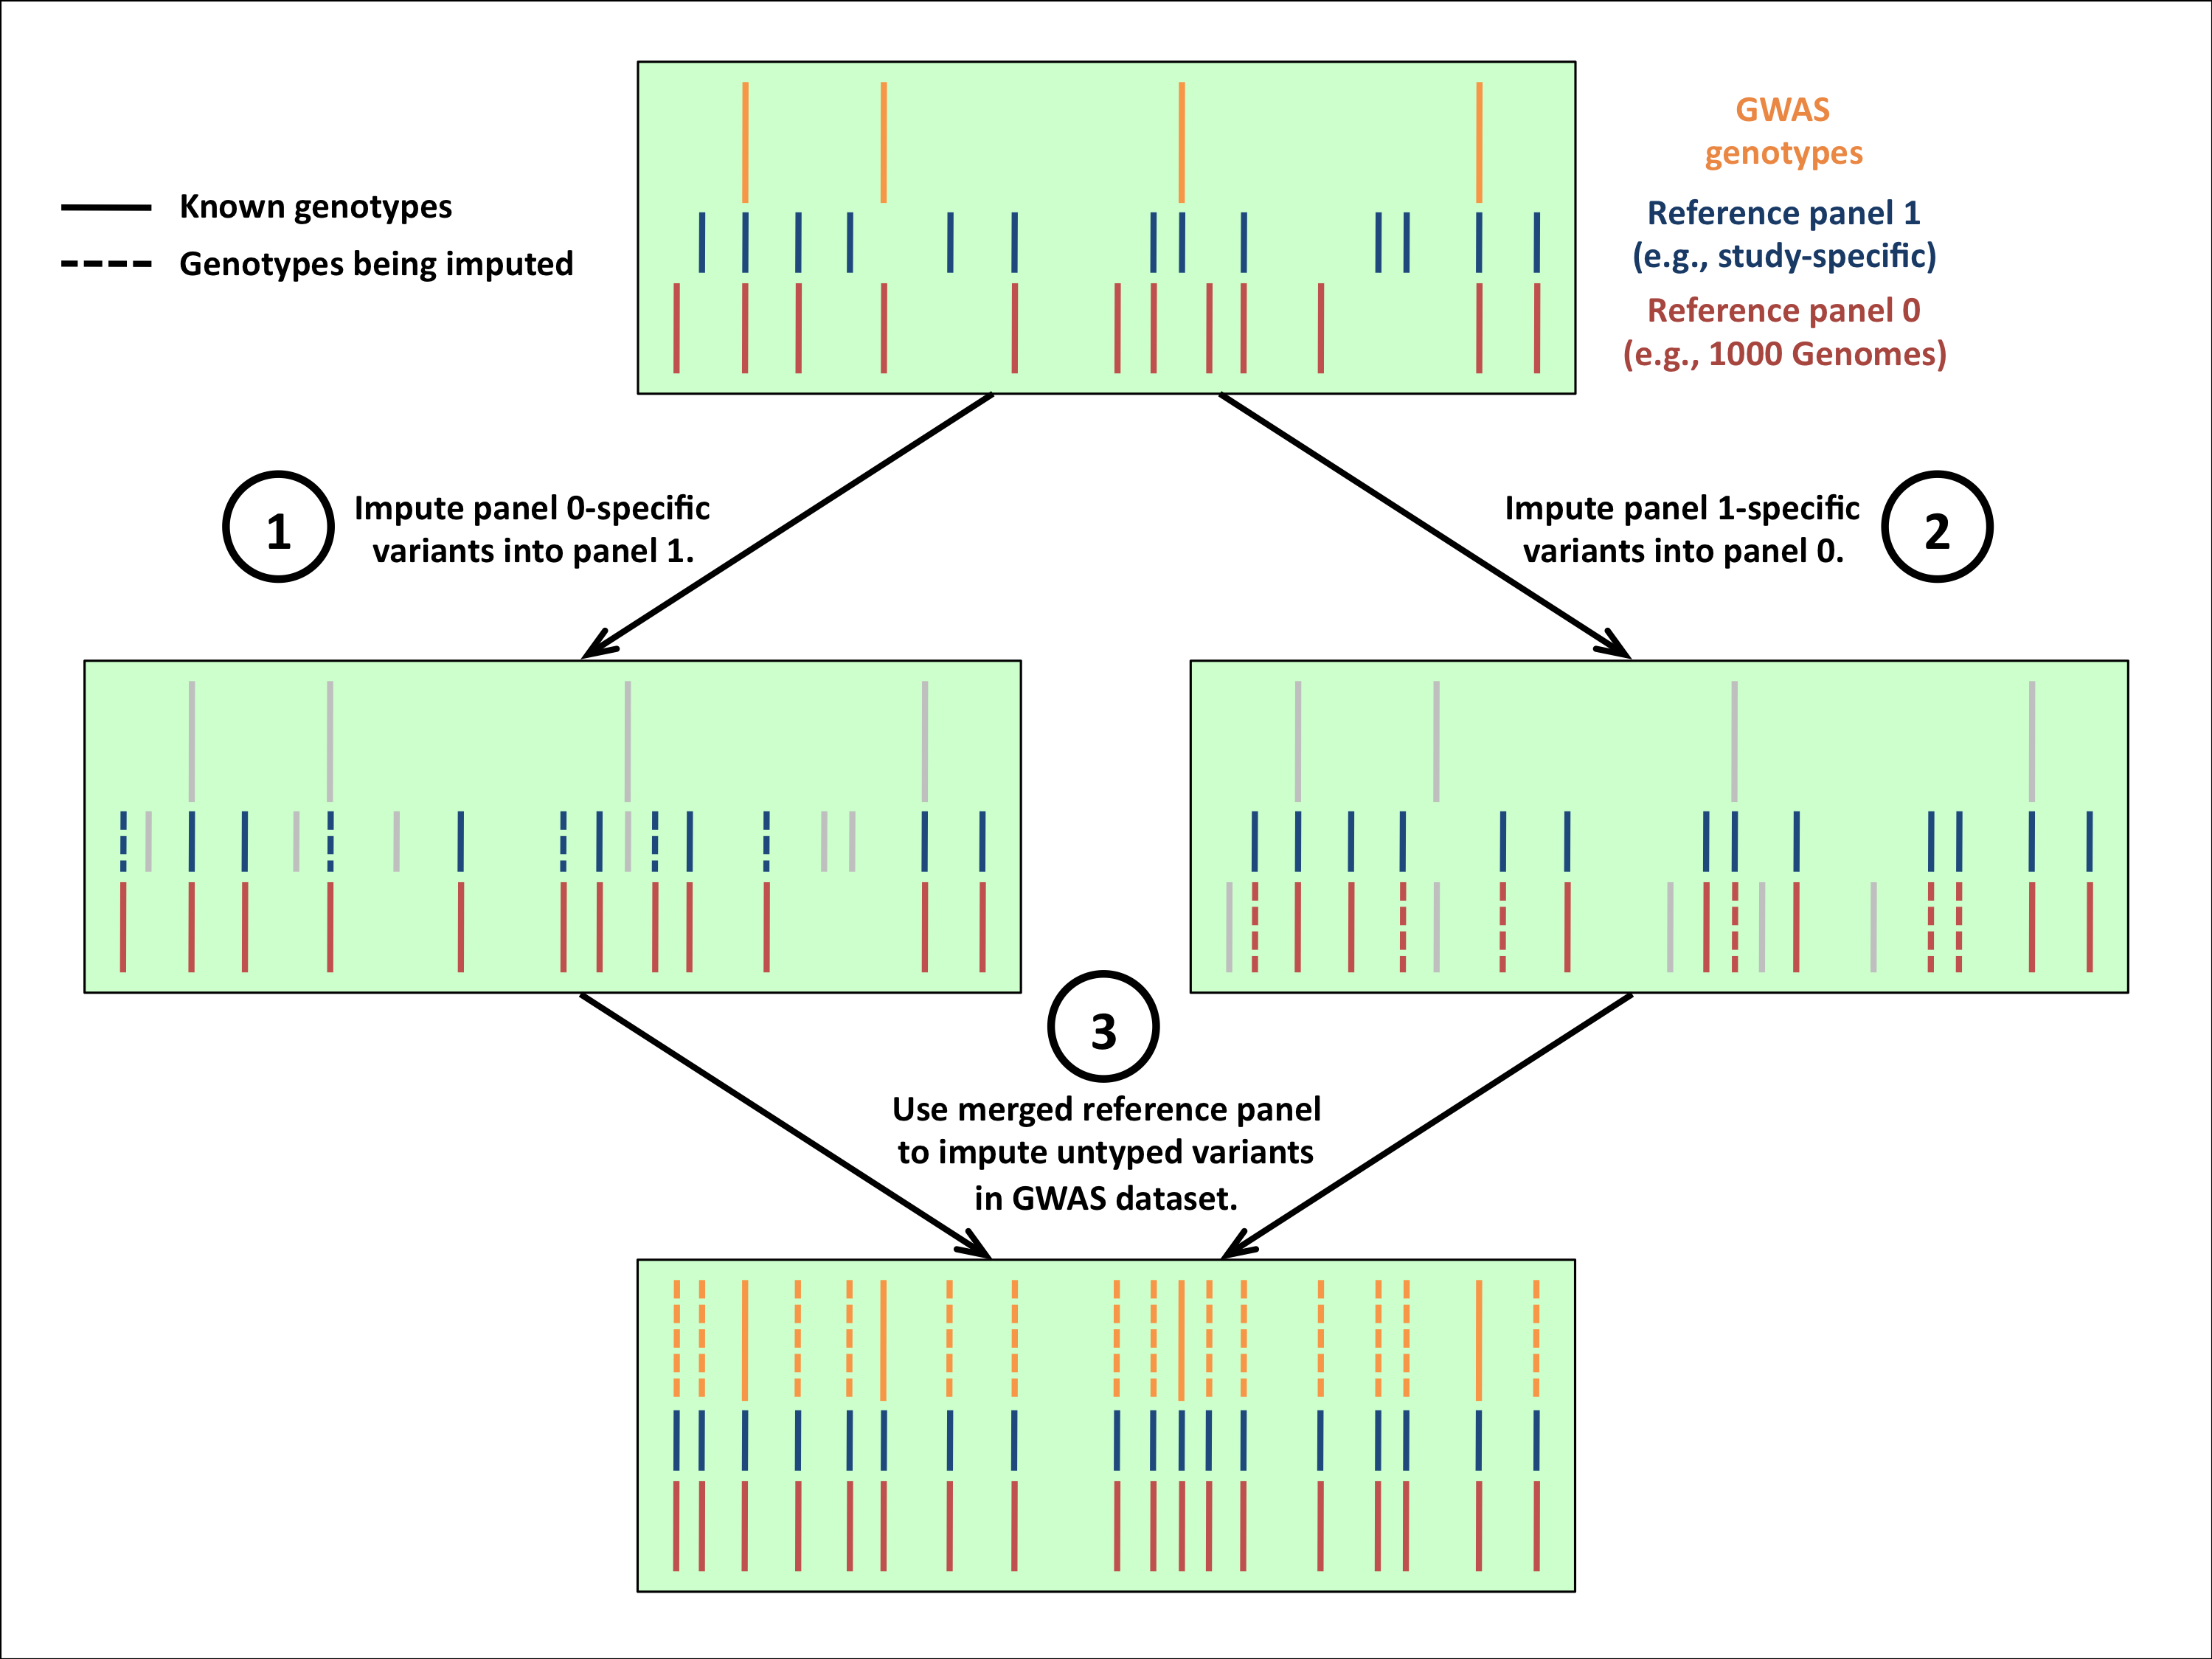
\includegraphics[width=0.6\textwidth]{merging_reference_panels}
\caption{The principle of creating a non-sparse matrix is the same as the merger of reference panels by imputation software. Figure copied from \href{http://mathgen.stats.ox.ac.uk/impute/merging\_reference\_panels.png}{IMPUTE2 web site}.}
\label{fig:merging_reference_panels}
\end{figure}

\subsection{Genotype refinement and phasing}
We carry out genotype refinement and phasing with SHAPEIT2.\cite{Delaneau2012} Initial refinement of genotype likelihoods is however carried out with Beagle4.\cite{Browning20071084} The posterior probabilities calculated by Beagle4 are then used as input for SHAPEIT2 along with a haplotype scaffold generated from SNP array data available for the same populations. The SNP array data undergoes QC per population and is phased with SHAPEIT2 across all populations to generate the haplotype scaffold.
%MVNcall can also utilize a haplotype scaffold and unlike SHAPEIT2 works for multiallelic sites.\cite{Menelaou2013} However, we use SHAPEIT2, because it improves on the accuracy of phasing.\cite{2014Delaneau}
The Illumina Omni2.5M SNP array has been shown to be an optimal/sufficient haplotype scaffold size in African populations.\cite{Menelaou2013}\cite{2014Delaneau} Pedigree information will be used by SHAPEIT2 when available. For Beagle4 this is less important, as this is only an initial refinement used as input for SHAPEIT2. We use the duoHMM method of SHAPEIT2 for phasing, because it has been shown to have a lower switch error rate, when pedigree information is available.\cite{OConnell2014} Following generation of this haplotype scaffold, SHAPEIT2 phases the sequence data by filling in missing data in between the scaffold, resulting in more accuracte phasing of sequence data.

The chip data will undergo calling and quality control as previously.\cite{Gurdasani2014}. For the haplotype scaffold, in addition to in-house genotype data available, we will also use called chip data from the 1000G populations YRI (Yoruba in Ibadan, Nigeria) and LWK (Luhya in Webuye, Kenya), which are the only African populations alongside MKK (Maasai in Kinyawa, Kenya), which were genotyped on the Illumina Omni2.5M chip as part of 1000G.
%ftp://ftp.1000genomes.ebi.ac.uk/vol1/ftp/release/20130502/supporting/hd_genotype_chip/

We use the latest release (1274) of Beagle4. We use a sliding window size of 50000 variants and an overlap of 3000 variants between sliding windows. We use the default parameters; e.g. singlescale=0.8, duoscale=1.0, trioscale=1.0, burnin-its=5, phase-its=5, impute-its=5. We sample 4 haplotypes for each individual during each iteration of the algorithm (nsamples=4) and use 1200 variants to build the haplotype frequency model at each locus (buildwindow=1200).

%Figure 8: Overall percent genotype discordance for different scaffold SNP density. Results are presented by population groups: African, European and Asian.
%Is MVNCall only better, if BEAGLE doesn't have phasing information?
%2014Delaneau - "It has been observed that the Beagle method does not have this property, and that Thunder and Impute2 benefit from using an initial set of haplotypes estimated via Beagle."
%2014Delaneu - "This approach generalizes our MVNcall, approach which is designed to phase one variant site at a time onto a haplotype scaffold, and improves upon its accuracy, by phasing multiple sites jointly onto the scaffold and using a more sophisticated underlying model."

%% https://mathgen.stats.ox.ac.uk/genetics_software/shapeit/shapeit.html#gcall

\subsection{Quality control after variant calling and genotype refinement}
If SNP array data is available, we further check after genotype refinement with Beagle4 that the concordance between chip and sequence genotypes is greater than 0.98 for each sample. We also check for heterozygosity outliers (\textgreater3SD) and PCA outliers after genotype refinement. Variant calling and genotype refinement is repeated if a sample either fails the check of genotype concordance, which is a sign of poor data quality, or fails the check of heterozygosity, which can be a sign of sample contamination or a population outlier.
\section{Merging of Datasets}

Following curation of individual datasets, these will need to be merged to homogenise variant calls across all data, and generate a square matrix of variant calls, where the union of variants across all samples is available for each population. In order to do this, a union set of calls will be generated for variants that have passed filtering in each dataset (Figure 1). Prior to merging 1) indels will be left aligned (e.g. bcftools norm), 2) SNPs and indels called in low coverage data by UnifiedGenotyper will be merged into single records with bcftools (bcftools norm -m +any) and 3) variants called from reads aligned to build 38 will be lifted over to build 37 (liftOver). %http://hgdownload.soe.ucsc.edu/admin/exe/linux.x86_64/liftOver
Variants will be merged across cohorts (GATK CombineVariants --minimalVCF or bcftools merge | bcftools view -G). These sites will then be recalled in each dataset to generate genotype likelihoods at these sites. Where necessary the union set of sites will be lifted over to build 38 prior to recalling and the recalled variants will then be lifted back over to build 37. UG and HC (--genotyping\_mode GENOTYPE\_GIVEN\_ALLELES) will be used for recalling of low and high coverage data, respectively. The maximum number of allowed alternate alleles will be increased from the default 6 by multiplication with the number of original cohorts to allow all true variants to be called.

Following this, genotype refinement will be carried out using Beagle4. For data with pedigree information, this information will be utilised in calling as well as phasing of data. Following refinement of genotype probabilities in Beagle, haplotype phasing will be carried out with SHAPEIT2 to maximise phasing accuracy, especially given the relatedness among some sample sets. MVNcall\cite{Menelaou2013} will then be applied where genotype information is available, within and outside pedigrees to further refine genotype calls based on generating a haplotype scaffold from the 2.5M Omni genotype data available on many sample sets.

\begin{figure}[h]
\caption{Homogenised calling across all datasets to generate a single panel}
\centering
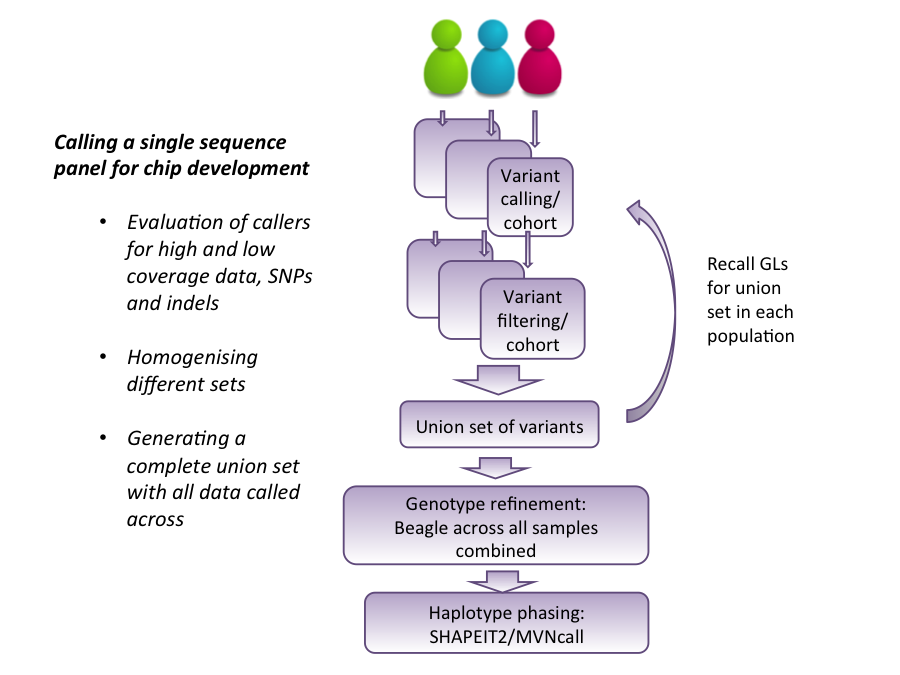
\includegraphics[width=0.8\textwidth]{calling}
\end{figure}

%\section{Evaluation of Variant Callers}
\subsection{Introduction}
We need to generate a set of high quality variants to be used in a reference panel and to be used as a set of candidate SNPs for tagSNP selection. Therefore it important to evaluate the various methods for calling variants such as SNPs, short indels and structural variants (SVs) for the sequence reads.
\subsection{Methods}
Variants ...
\section{Identification of Informative Variants for the Chip Array}

For identification of informative variants on the chip array, we will utilise a hybrid algorithm with cycles of LD based pairwise tagging, and imputation, as has been previously described.\cite{} Only populations with at least 50 samples will be included in the chip design process, as pairwise LD evaluation would be difficult in smaller samples. Here, the term ‘population’ should be considered distinct from an ethno-linguistic group/project, and constitutes a group of individuals/samples that appear genetically homogeneous, without any significant substructure or clustering. In order to account for different sample sizes and LD differentiation among populations, we will carry out multi-population pairwise tagging, as described below. We seek only to tag common SNPs (MAF\textgreater5\%) for generation of this array.

We have developed a multi-population tagging algorithm based on the algorithm TAGster for WGS data.\cite{Xu2007} The methods we used for tagging were identical to those used by TAGster; however, by using seeking and indexing approaches we were able to optimise the computational efficiency of the algorithm by an order of magnitude (unpublished data, Carstensen et al.). We briefly outline the tagging algorithm as follows (Figure 2):

\begin{enumerate}
\item Calculate LD (\textit{r}\textsuperscript{2}) between each SNP and all other SNPs in the flanking 250 KB region for each population separately. MAF thresholds are imposed at this stage, and only pairs of SNPs where both exceed the MAF threshold are included.
\item For each SNP not already in the tagging set, a count of SNPs in the target set that are in LD exceeding a given threshold \textit{r}\textsuperscript{2} with it is generated across the genome and summed across all populations.
\item The most informative SNP (the SNP with most target SNPs in LD with it summed across population) is chosen as the tagging SNP and added to the set of tagging SNPs.
\item This tagging SNP and SNPs in LD with it are now removed from the set of target SNPs. This process is carried out separately for each population, so that a separate set of target SNPs is maintained for each population set. However, SNPs in LD with the tagging SNP can still be picked up as tagging SNPs themselves if they independently tag the maximum no. of SNPs in any iteration.
Steps 2-3 are repeated until either a specified number of SNPs or all target SNPs (chosen as SNPs above a specific MAF threshold per-population) are tagged across all population sets, or until a specific number of SNPs is reached, as specified.
\end{enumerate}

\begin{figure}[h]
\caption{Hybrid tagging and imputation algorithm for chip design.}
\centering

\includegraphics[width=0.8\textwidth]{tagSNPselection}
\end{figure}

Although this method works well across populations, it only carries out pairwise single-marker tagging. Haplotype based, or multi-marker tagging would potentially be more efficient, and select fewer tagging sites. In order to incorporate haplotype based tagging into our model, we use a hybrid method, with cycles of tagging and imputation, as has been described before.2 

In order to implement this method, in the first cycle, we select a maximum number of pre-defined tagging SNPs. Following this, these tagging SNPs are selected from each population, and imputation is carried out using a reference panel, to identify additional sites in each population that are tagged at an $r^{2}$ threshold above 0.80 by the tagging sites. These sites are removed from the target set for each population, and do not contribute to the next cycle, thereby making the process more efficient. For imputation, we include the entire reference panel curated from all samples in table \ref{table:samples}, including the 1000 Genomes multi-ethnic samples from Europe, Asian and the Americas, to maximise imputation accuracy. However, for imputation into each population, samples from the given population are removed from the reference set, so the imputation panel does not include any samples from the population being evaluated for tagging. This ‘leave one population out’ approach would produce relatively conservative results for tagging, with more variants being tagged than if a subsample of the population was included in the reference panel. This is a more realistic scenario, as it is not necessary that any given population genotyped on the chip in future would be represented in the reference panel.

Additionally, pre-selected known biologically relevant variants, valuable to the studies planned for consortia can be included on the array, to replace certain tag SNPs. We have previously shown that a 1M tagging variants chosen using the described algorithm can produce \textgreater80\% coverage across diverse populations in Africa. Based on this, we plan to carry out approximately 10 cycles to capture 1.2M tagging variants, in order to prioritise variants to include in the design of a 1M chip array. Following this, we will further validate our tagging algorithm among populations with smaller sample sizes that were not included in the development in the chip array, by selecting tagging variants among these and imputing with the reference panel, excluding these populations. We estimate coverage of each population by such a chip array using imputation. Coverage is defined as the proportion of common variation captured at an r2>0.80 across the genome in a given population with the combined reference panel (excluding the population being evaluated). $r^{2}$, here, is calculated as the correlation between the sequence data and imputed data on a hypothetical 1M chip array for common variation. 

\section{Evaluation of variant callers}

In order to explore the sensitivity and specificity of variant callers when applied to low coverage datasets, we carried out an evaluation with 1,986 samples from Uganda sequenced at 4x average coverage with Illumina HiSeq 2000. The down-sampled GiaB sample\cite{Zook2014} (6x) was included in the called set for validation. We calculated the sensitivity and specificity of calls relative to the highly curated variant sites for the NA12878 sample, to identify the caller with greatest area under ROC curve at different filtering thresholds (Figure 3). We used two different filtering thresholds for this analysis: the SNP quality metric (QUAL), and the VQSLOD score obtained using the VQSR model implemented by GATK for different callers. With this evaluation, we show that UnifiedGenotyper3.2 shows the best area under ROC curve with the lowest FDR for a given sensitivity for SNPs and indels (Figure \ref{fig:roc}). All callers, however produce very low sensitivity and high FDRs for indel calls (Figure \ref{fig:roc_indels}). It is likely that the sensitivity and specificity of calls will improve with genotype refinement, particularly when carried out along with high coverage data from X10 sequencing. Variant Quality score recalibration (VQSR) based filtering approaches seem to perform better than filtering only on variant quality for most calls. However, further exploration of filtering approaches for indel calls is needed, including appropriate normalisation of model training sets, as this could potentially improve the sensitivity for a given FDR. Additionally, a new release of HaplotypeCaller corrects issues with previous releases, potentially greatly improving the sensitivity for SNPs and indels. A comparison of these callers with consistent filtering methods will inform the best method to use for calling SNPs and indels within low coverage (4x) data. Choosing appropriate callers and filtering methods is crucial maximising variant discovery while maintaining low false discovery on the panel curated for the development of the chip array.

\begin{figure}[h]
\captionsetup{width=0.8\textwidth}
\caption{An evaluation of calling algorithms for SNPs and indels in low coverage data. The figure depicts a comparison of various calling algorithms using different filters for calling SNPs (left) and indels (right) in low coverage data. The x axis represents the false discovery rate (FDR), which is defined as the proportion of calls produced by a given algorithm that are false positives at a given filtering threshold. The y axis represents the true positive rate or the sensitivity, which is the proportion of all true calls in the GiaB sample that are captured by a given algorithm for a given filtering threshold. The curves are generated by varying filtering thresholds for each algorithm. UG: UnifiedGenotyper; FB: FreeBayes; HC: HaplotypeCaller; QUAL: Phred-scaled quality score; VQSLOD: Variant Quality Recalibration scores; NIST: National Institute of Standards and Technology.}
\label{fig:roc}
\centering
    \begin{subfigure}[b]{0.45\textwidth}
        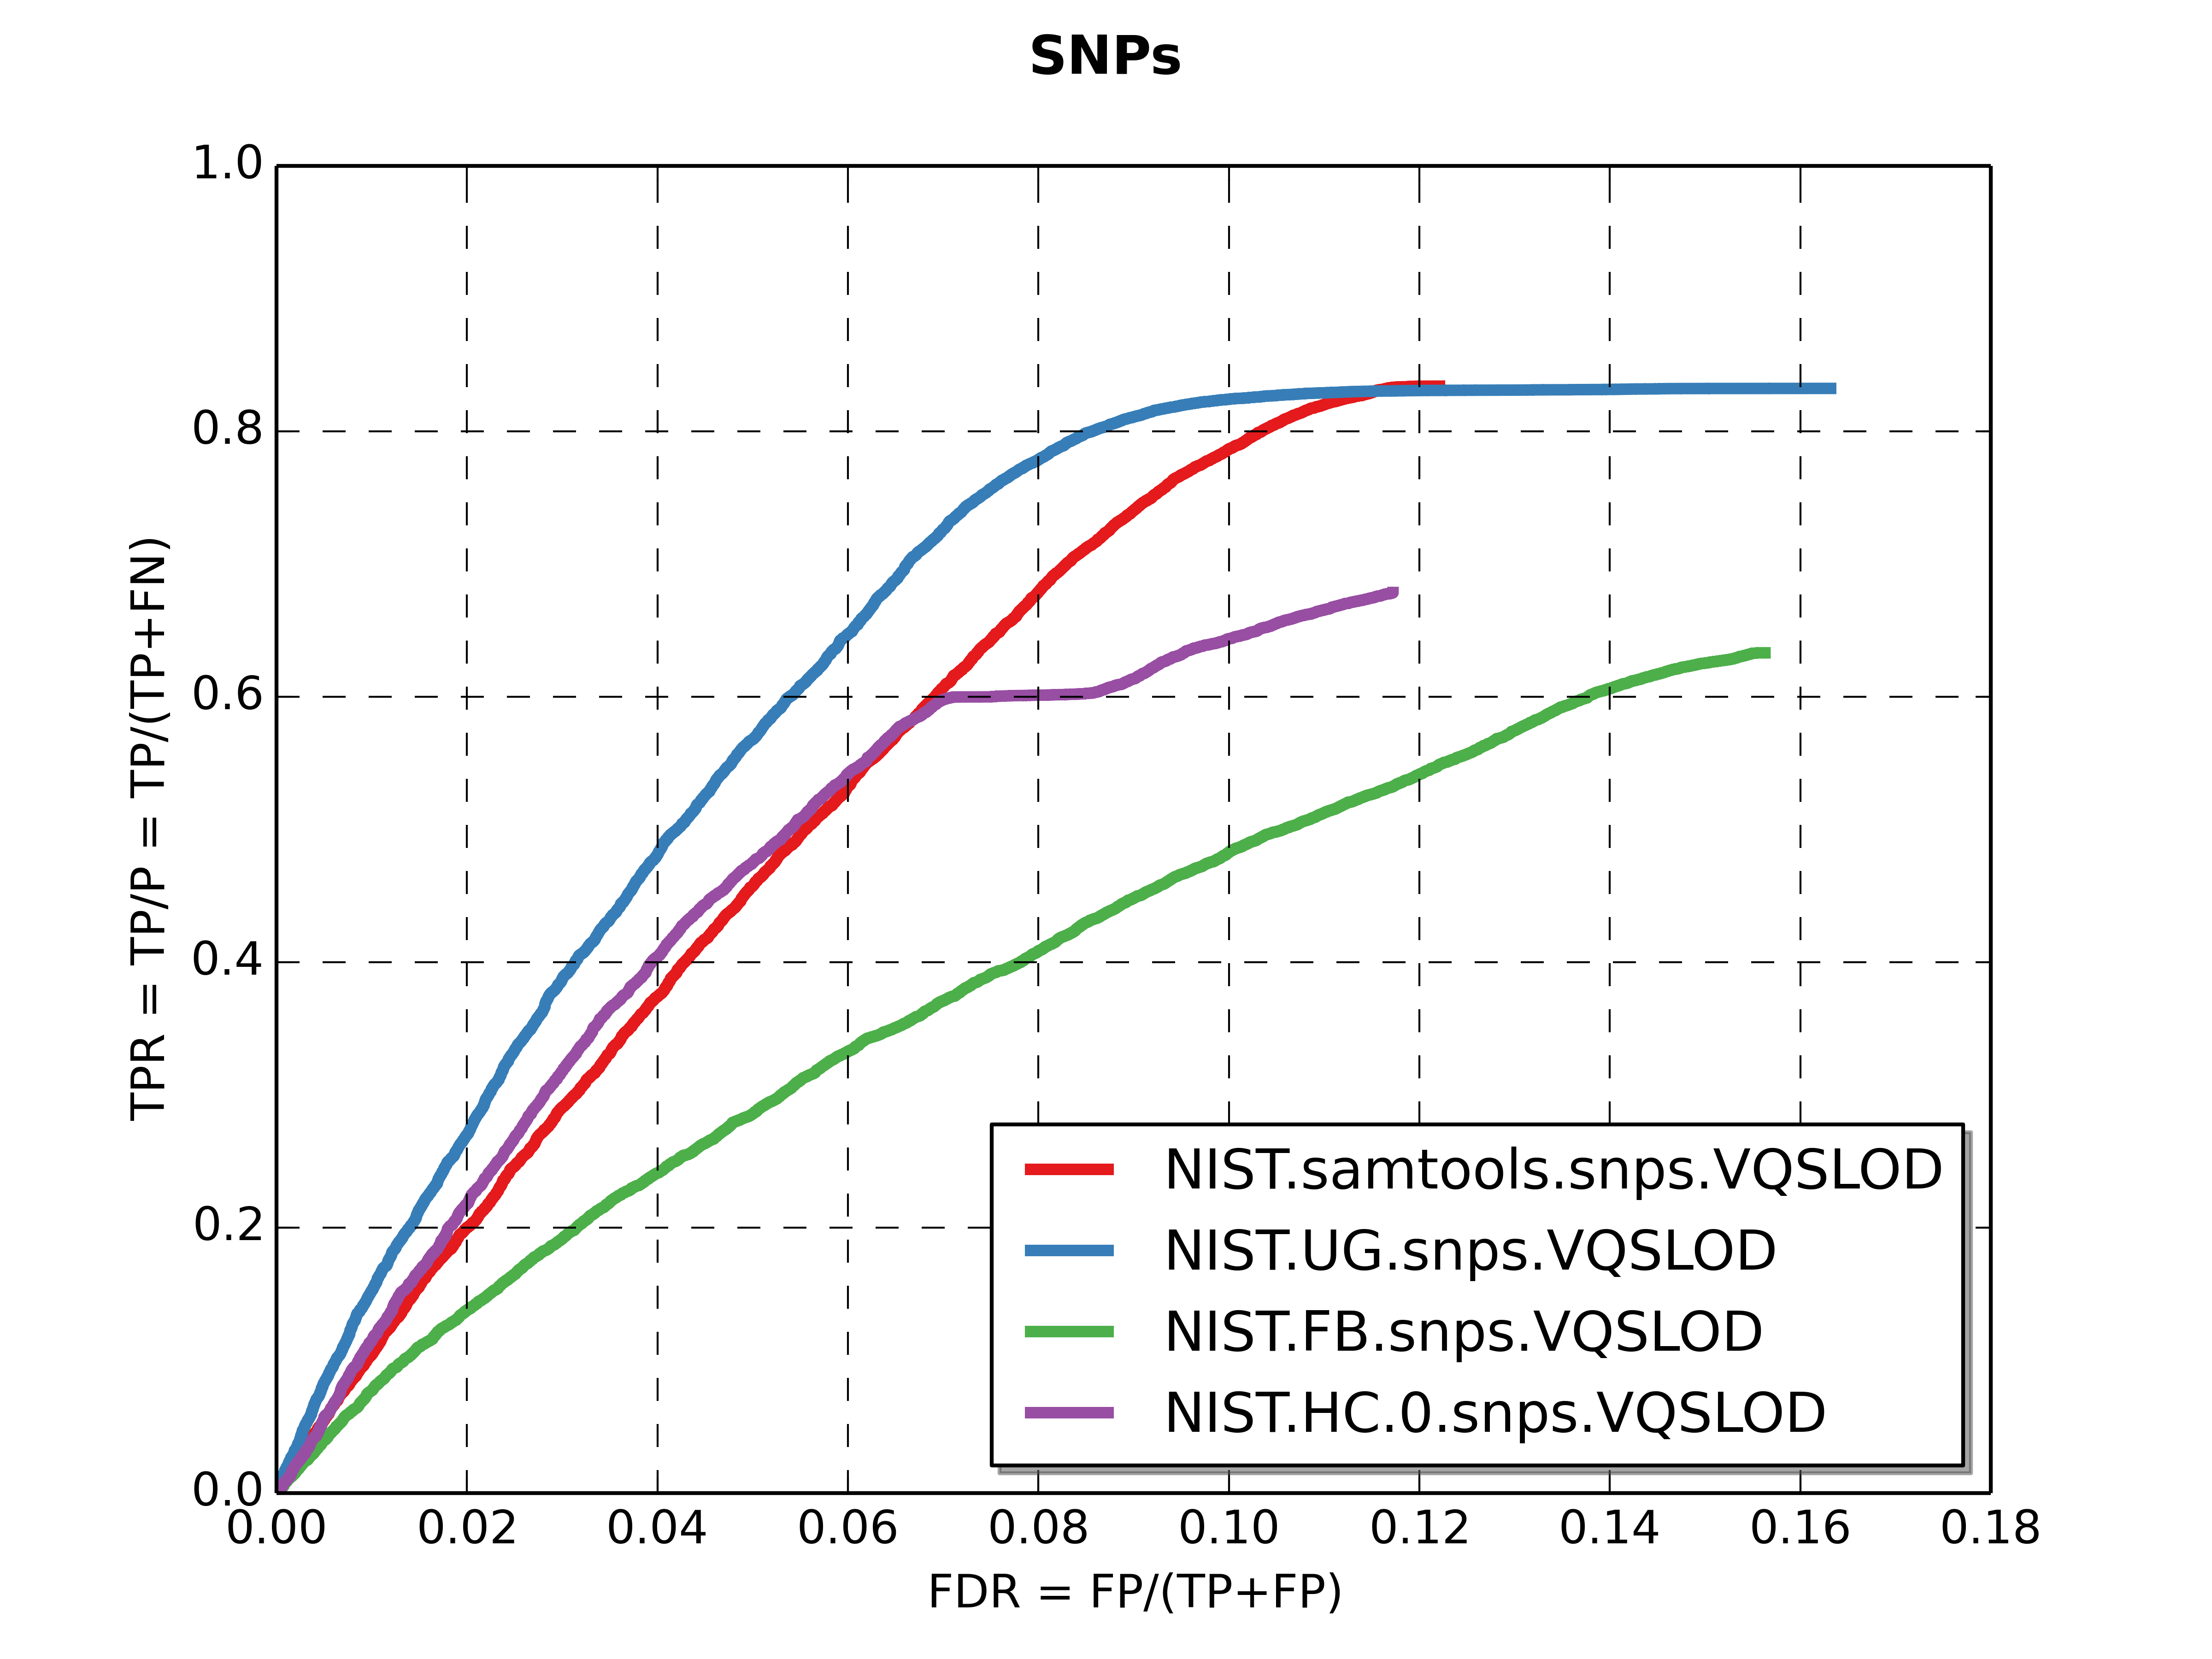
\includegraphics[width=\textwidth]{FDR_snps}
        \caption{SNPs}
        \label{fig:roc_snps}
    \end{subfigure}%
    \begin{subfigure}[b]{0.45\textwidth}
        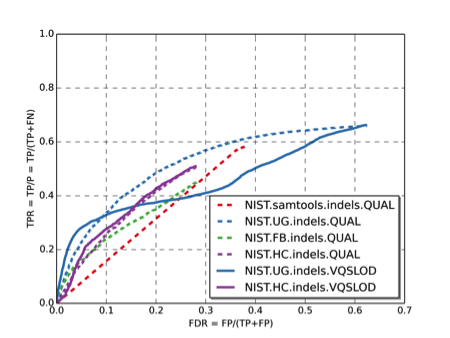
\includegraphics[width=\textwidth]{FDR_indels}
        \caption{Indels}
        \label{fig:roc_indels}
    \end{subfigure}%
\end{figure}

For high coverage data, we evaluated the NA12878 sample alone re-sequenced on the X-10 pipeline with the highly curated set of variants produced by GiaB.1 We showed that the X-10 and the new pipeline used with it produced high quality data that when normalised showed a high degree of sensitivity versus the GiaB reference set and a low false discovery rate (Table \ref{table:highcoverage}). When the Illumina 50x Platinum set, sequenced on the Illumina Hiseq 2000 platform was reprocessed through the same pipeline it produced similarly high results, though the INDEL sensitivity and false discovery rate were slightly better. We believe this may be because of the higher coverage and PCR free library preparation used in the creation of this sequence.

\begin{table}[h]
\centering
%\resizebox{\textwidth}{!}{%
\begin{tabular}{l|lrrrrr}
\rowcolor[HTML]{333333} 
{\color[HTML]{FFFFFF} Sample} & {\color[HTML]{FFFFFF} Type} & {\color[HTML]{FFFFFF} TP} & {\color[HTML]{FFFFFF} FP} & {\color[HTML]{FFFFFF} FN} & {\color[HTML]{FFFFFF} Sensitivity} & {\color[HTML]{FFFFFF} FDR} \\
 & \cellcolor[HTML]{C0C0C0}SNP & \cellcolor[HTML]{C0C0C0}2914294 & \cellcolor[HTML]{C0C0C0}28213 & \cellcolor[HTML]{C0C0C0}10266 & \cellcolor[HTML]{C0C0C0}0.9965 & \cellcolor[HTML]{C0C0C0}0.0096 \\
\multirow{-2}{*}{Replicate 1} & INDEL & 413639 & 23145 & 34743 & 0.9255 & 0.0530 \\
 & \cellcolor[HTML]{C0C0C0}SNP & \cellcolor[HTML]{C0C0C0}2908260 & \cellcolor[HTML]{C0C0C0}26311 & \cellcolor[HTML]{C0C0C0}14452 & \cellcolor[HTML]{C0C0C0}0.9951 & \cellcolor[HTML]{C0C0C0}0.0090 \\
\multirow{-2}{*}{Replicate 2} & INDEL & 393431 & 24110 & 52542 & 0.8822 & 0.0577 \\
 & \cellcolor[HTML]{C0C0C0}SNP & \cellcolor[HTML]{C0C0C0}2917290 & \cellcolor[HTML]{C0C0C0}21400 & \cellcolor[HTML]{C0C0C0}9844 & \cellcolor[HTML]{C0C0C0}0.9966 & \cellcolor[HTML]{C0C0C0}0.0073 \\
\multirow{-2}{*}{Platinum} & INDEL & 437875 & 8802 & 2297 & 0.9948 & 0.0197
\end{tabular}
%}
\caption{Intersect of NA12878 samples with GiaB reference calls version 0.2.}
\label{table:FDRhigh}
\end{table}
\section{Validation of selected tag SNPs}

As sequence data, particularly low coverage short read data has been prone to sequencing errors, we will validate all tagging sites based on a large data repository of validated variant sites collated by Affymetrix. Novel variant sites will be further validated by Affymetrix, prior to chip design, and proxies of sites that cannot be covered will be investigated and filled in for generation of the final array.

\bibliographystyle{unsrt}%Used BibTeX style is unsrt
\bibliography{references/references}

%We don't filter based on the percentage of mapped reads. Instead we filter based on heterozygosity. The two parameters are related.

%“Version 4 has multiple improvements: support for multi-allelic markers” – BEAGLE4 site

%An improved method for calling genotypes and phasing low-coverage data when one also has chip data is to phase the chip data to make a haplotype scaffold and then phase the sequence data onto the scaffold. Both steps are carried out with SHAPEIT2.

\end{document}
